% !TeX encoding = UTF-8
% !TeX program = xelatex
% !TeX spellcheck = en_US

\documentclass[degree=bachelor]{thuthesis}
  % 学位 degree:
  %   doctor | master | bachelor | postdoc
  % 学位类型 degree-type:
  %   academic(默认)| professional
  % 语言 language
  %   chinese(默认)| english
  % 字体库 fontset
  %   windows | mac | fandol | ubuntu
  % 建议终版使用 Windows 平台的字体编译


% 论文基本配置,加载宏包等全局配置
% !TeX root = ./thuthesis-example.tex

% 论文基本信息配置

\thusetup{
  %******************************
  % 注意:
  %   1. 配置里面不要出现空行
  %   2. 不需要的配置信息可以删除
  %   3. 建议先阅读文档中所有关于选项的说明
  %******************************
  %
  % 输出格式
  %   选择打印版(print)或用于提交的电子版(electronic),前者会插入空白页以便直接双面打印
  %
  output = print,
  %
  % 标题
  %   可使用“\\”命令手动控制换行
  %
  title  = {清华大学学位论文 \LaTeX{} 模板\\使用示例文档 v\version},
  title* = {An Introduction to \LaTeX{} Thesis Template of Tsinghua
            University v\version},
  %
  % 学位
  %   1. 学术型
  %      - 中文
  %        需注明所属的学科门类,例如:
  %        哲学、经济学、法学、教育学、文学、历史学、理学、工学、农学、医学、
  %        军事学、管理学、艺术学
  %      - 英文
  %        博士:Doctor of Philosophy
  %        硕士:
  %          哲学、文学、历史学、法学、教育学、艺术学门类,公共管理学科
  %          填写“Master of Arts“,其它填写“Master of Science”
  %   2. 专业型
  %      直接填写专业学位的名称,例如:
  %      教育博士、工程硕士等
  %      Doctor of Education, Master of Engineering
  %   3. 本科生不需要填写
  %
  degree-name  = {工学硕士},
  degree-name* = {Master of Science},
  %
  % 培养单位
  %   填写所属院系的全名
  %
  department = {计算机科学与技术系},
  %
  % 学科
  %   1. 学术型学位
  %      获得一级学科授权的学科填写一级学科名称,其他填写二级学科名称
  %   2. 工程硕士
  %      工程领域名称
  %   3. 其他专业型学位
  %      不填写此项
  %   4. 本科生填写专业名称,第二学位论文需标注“(第二学位)”
  %
  discipline  = {计算机科学与技术},
  discipline* = {Computer Science and Technology},
  %
  % 姓名
  %
  author  = {薛瑞尼},
  author* = {Xue Ruini},
  %
  % 指导教师
  %   中文姓名和职称之间以英文逗号“,”分开,下同
  %
  supervisor  = {郑纬民, 教授},
  supervisor* = {Professor Zheng Weimin},
  %
  % 副指导教师
  %
  associate-supervisor  = {陈文光, 教授},
  associate-supervisor* = {Professor Chen Wenguang},
  %
  % 联合指导教师
  %
  % co-supervisor  = {某某某, 教授},
  % co-supervisor* = {Professor Mou Moumou},
  %
  % 日期
  %   使用 ISO 格式;默认为当前时间
  %
  % date = {2019-07-07},
  %
  % 是否在中文封面后的空白页生成书脊(默认 false)
  %
  include-spine = false,
  %
  % 密级和年限
  %   秘密, 机密, 绝密
  %
  % secret-level = {秘密},
  % secret-year  = {10},
  %
  % 博士后专有部分
  %
  % clc                = {分类号},
  % udc                = {UDC},
  % id                 = {编号},
  % discipline-level-1 = {计算机科学与技术},  % 流动站(一级学科)名称
  % discipline-level-2 = {系统结构},          % 专业(二级学科)名称
  % start-date         = {2011-07-01},        % 研究工作起始时间
}

% 载入所需的宏包

% 定理类环境宏包
\usepackage{amsthm}
% 也可以使用 ntheorem
% \usepackage[amsmath,thmmarks,hyperref]{ntheorem}

\thusetup{
  %
  % 数学字体
  % math-style = GB,  % GB | ISO | TeX
  math-font  = xits,  % stix | xits | libertinus
}

% 可以使用 nomencl 生成符号和缩略语说明
% \usepackage{nomencl}
% \makenomenclature

% 表格加脚注
\usepackage{threeparttable}

% 表格中支持跨行
\usepackage{multirow}

% 固定宽度的表格。
% \usepackage{tabularx}

% 跨页表格
\usepackage{longtable}

% 算法
% \usepackage{algorithm}
\usepackage[ruled, vlined, linesnumbered, commentsnumbered, longend]{algorithm2e} % changed by Colin

% 量和单位
\usepackage{siunitx}

% 参考文献使用 BibTeX + natbib 宏包
% 顺序编码制
% \usepackage[sort]{natbib}
% \bibliographystyle{thuthesis-numeric}

% 著者-出版年制
% \usepackage{natbib}
% \bibliographystyle{thuthesis-author-year}

% 本科生参考文献的著录格式
\usepackage[sort]{natbib}
\bibliographystyle{thuthesis-bachelor}

% 参考文献使用 BibLaTeX 宏包
% \usepackage[style=thuthesis-numeric]{biblatex}
% \usepackage[style=thuthesis-author-year]{biblatex}
% \usepackage[style=apa]{biblatex}
% \usepackage[style=mla-new]{biblatex}
% 声明 BibLaTeX 的数据库
% \addbibresource{ref/refs.bib}

% 定义所有的图片文件在 figures 子目录下
\graphicspath{{figures/}}

% force line breaks in a cell
\usepackage{makecell}

% 数学命令
\makeatletter
\newcommand\dif{%  % 微分符号
  \mathop{}\!%
  \ifthu@math@style@TeX
    d%
  \else
    \mathrm{d}%
  \fi
}
\makeatother

% \usepackage[outputdir=../]{minted}
\usepackage{minted}
\usemintedstyle{manni}

% \usepackage{svg}

% quote
\newcommand*\openquote{\makebox(15,-20){\scalebox{5}{``}}}
\newcommand*\closequote{\makebox(15,-20){\scalebox{5}{''}}}
\definecolor{azure}{rgb}{0.94, 1.0, 1.0}
\colorlet{shadecolor}{azure}
\newenvironment{myquote}[1]%
  {\list{}{\leftmargin=#1\rightmargin=#1}\item[]}%
  {\endlist}
  
\makeatletter
\newif\if@right
\def\shadequote{\@righttrue\shadequote@i}
\def\shadequote@i{\begin{snugshade}\begin{myquote}{1cm}}
\def\endshadequote{%
  \if@right\hfill\fi\end{myquote}\end{snugshade}}
\@namedef{shadequote*}{\@rightfalse\shadequote@i}
\@namedef{endshadequote*}{\endshadequote}
\makeatother

% hyperref 宏包在最后调用
\usepackage{hyperref}


\thusetup{
    title = {基于混合算子计算图生成的深度学习编译器模糊测试},
    % title* = {Improving fuzz testing for deep learning compilers},
    department = {计算机科学与技术系},
    discipline = {计算机科学与技术},
    author = {彭晋钧},
    supervisor = {韩文弢, 讲师},
    co-supervisor = {},
    associate-supervisor = {},
    % date = {2011-07-01},
}

\begin{document}

% 封面
\maketitle

% 学位论文指导小组、公开评阅人和答辩委员会名单
% 本科生不需要
% % !TeX root = ../thuthesis-example.tex

\begin{committee}[name={学位论文指导小组、公开评阅人和答辩委员会名单}]

  \newcolumntype{C}[1]{@{}>{\centering\arraybackslash}p{#1}}

  \section*{指导小组名单}

  \begin{center}
    \begin{tabular}{C{3cm}C{3cm}C{9cm}@{}}
      李XX & 教授     & 清华大学 \\
      王XX & 副教授   & 清华大学 \\
      张XX & 助理教授 & 清华大学 \\
    \end{tabular}
  \end{center}


  \section*{公开评阅人名单}

  \begin{center}
    \begin{tabular}{C{3cm}C{3cm}C{9cm}@{}}
      刘XX & 教授   & 清华大学                    \\
      陈XX & 副教授 & XXXX大学                    \\
      杨XX & 研究员 & 中国XXXX科学院XXXXXXX研究所 \\
    \end{tabular}
  \end{center}


  \section*{答辩委员会名单}

  \begin{center}
    \begin{tabular}{C{2.75cm}C{2.98cm}C{4.63cm}C{4.63cm}@{}}
      主席 & 赵XX                  & 教授                    & 清华大学       \\
      委员 & 刘XX                  & 教授                    & 清华大学       \\
          & \multirow{2}{*}{杨XX} & \multirow{2}{*}{研究员} & 中国XXXX科学院 \\
          &                       &                         & XXXXXXX研究所  \\
          & 黄XX                  & 教授                    & XXXX大学       \\
          & 周XX                  & 副教授                  & XXXX大学       \\
      秘书 & 吴XX                  & 助理研究员              & 清华大学       \\
    \end{tabular}
  \end{center}

\end{committee}



% 也可以导入 Word 版转的 PDF 文件
% \begin{committee}[file=figures/committee.pdf]
% \end{committee}


% 使用授权的说明
\copyrightpage
% 将签字扫描后授权文件 scan-copyright.pdf 替换原始页面
% \copyrightpage[file=scan-copyright.pdf]

\frontmatter
% !TeX root = ../thuthesis-example.tex

% 中英文摘要和关键字

\begin{abstract}

深度学习编译器是将神经网络模型部署到特定硬件平台上并进行优化的核心工具,其正确性对提高神经网络实际应用的可靠性至关重要。
近年来,已有研究者利用软件工程领域中寻找程序漏洞的常用技术——模糊测试,通过生成大量包含单个或多个算子的测试用例,结合差分测试,寻找深度学习编译器中的实现错误。然而,这些已有工作所生成测例的多样性仍存在提升空间,未能触发编译器中尽可能多的优化逻辑,以实现充分测试。

面对上述问题,在方法上,本课题提出符号化计算图生成这一已有算法的一种改进策略,通过引入具体化算子进行混合计算图生成,提高了模糊测试用例中计算图的多样性。实验表明,对于 PyTorch 与 TensorFlow 两种主流框架,该方法可以分别提高分支覆盖率 14.9\% 、 23.5\% ,研究过程中累计提交漏洞 62 个、 14 个,且在测例多样性与实际意义两方面均具有明显优势。
同时,本课题提出了一套在具体算子数据集上进行分类的规则,为基于自动规则与约束推导进行测例生成的未来工作奠定了基础。

在工程上,本课题基于前人已有的开源项目 NNSmith 进行拓展,不仅实现了上述方法中的具体算子收集与分类以及混合计算图生成,而且实现了模型的 Python 代码描述与图结构中间表示的相互转换,从而提高了测例的有效性,并为充分利用已有代码提供了实现基础。本课题的核心功能已经在 GitHub 上被提交与整合至 NNSmith 仓库,为后续研究的跟进与实际场景中的应用提供了便利。

在经验上,本课题呈现了深度学习编译器实现中的典型错误,并分析了触发它们的根因,直观体现了深度学习模糊测试框架的意义,与机器学习系统可靠性研究的重要性。
  
  % 论文的摘要是对论文研究内容和成果的高度概括。
  % 摘要应对论文所研究的问题及其研究目的进行描述,对研究方法和过程进行简单介绍,对研究成果和所得结论进行概括。
  % 摘要应具有独立性和自明性,其内容应包含与论文全文同等量的主要信息。
  % 使读者即使不阅读全文,通过摘要就能了解论文的总体内容和主要成果。

  % 论文摘要的书写应力求精确、简明。
  % 切忌写成对论文书写内容进行提要的形式,尤其要避免“第 1 章……;第 2 章……;……”这种或类似的陈述方式。

  % 关键词是为了文献标引工作、用以表示全文主要内容信息的单词或术语。
  % 关键词不超过 5 个,每个关键词中间用分号分隔。

  % 关键词用“英文逗号”分隔,输出时会自动处理为正确的分隔符
\thusetup{
  keywords = {深度学习编译器, 计算图, 测例生成, 模糊测试, 差分测试},
}
\end{abstract}

\begin{abstract*}
Deep learning compiler is a core tool to deploy neural network models to specific hardware platforms and optimize them, and its correctness is crucial to improve the reliability of neural network applications.
In recent years, some researchers have used the common technology of finding program bugs in the field of software engineering, fuzzing, to find implementation errors in deep learning compilers by generating a large number of test cases containing single or multiple operators and combining differential testing. However, the diversity of the generated test cases still has room for improvement, and the optimization logic in the compiler has not been triggered as much as possible to achieve sufficient testing.

Facing the problems above, in terms of method, we extend the existing graph generation algorithm, symbolic graph generation, by introducing concrete operators for hybrid graph generation, which improves the diversity of computation graphs in fuzzing test cases.
Experiments show that for the two commonly used frameworks, PyTorch and TensorFlow, our method can respectively improve the branch coverage by 14.9\% and 23.5\%, and submit 62 and 14 bugs or vulnerabilities in the research process, with advantages in both test case diversity and practical significance.
Meanwhile, we propose a set of rules for classification on the concrete operator dataset, which lays the foundation for future work on test case generation based on automatic rule and constraint inference.

In terms of engineering, we extend the existing open source project NNSmith. We not only implement the collection and classification of concrete operators as well as the hybrid computation graph generation, but also implement the mutual conversion between the Python code description of the model and the intermediate representation of the graph, which enhances the effectiveness of the test case and provides an implementation basis for making full use of existing code from other sources.
The core functions of this project have been merged into the NNSmith repository on GitHub, which provides convenience for follow-up research and application in real scenarios.

Empirically, we demonstrate typical bugs hidden behind deep learning compilers and analyze their root causes, intuitively presenting the significance of fuzzing deep learning frameworks and the importance of reliability research on modern machine learning systems. 

% Use comma as separator when inputting
\thusetup{
  keywords* = {Deep Learning Compiler, Computation Graph, Test Case Generation, Fuzzing, Differential Testing},
}
\end{abstract*}


% 目录
\tableofcontents


% 正文部分
\mainmatter
% !TeX root = ../thuthesis-example.tex

\chapter{论文主要部分的写法}

研究生学位论文撰写,除表达形式上需要符合一定的格式要求外,内容方面上也要遵循一些共性原则。

通常研究生学位论文只能有一个主题(不能是几块工作拼凑在一起),该主题应针对某学科领域中的一个具体问题展开深入、系统的研究,并得出有价值的研究结论。
学位论文的研究主题切忌过大,例如,“中国国有企业改制问题研究”这样的研究主题过大,因为“国企改制”涉及的问题范围太广,很难在一本研究生学位论文中完全研究透彻。



\section{论文的语言及表述}

除国际研究生外,学位论文一律须用汉语书写。
学位论文应当用规范汉字进行撰写,除古汉语研究中涉及的古文字和参考文献中引用的外文文献之外,均采用简体汉字撰写。

国际研究生一般应以中文或英文书写学位论文,格式要求同上。
论文须用中文封面。

研究生学位论文是学术作品,因此其表述要严谨简明,重点突出,专业常识应简写或不写,做到立论正确、数据可靠、说明透彻、推理严谨、文字凝练、层次分明,避免使用文学性质的或带感情色彩的非学术性语言。

论文中如出现一个非通用性的新名词、新术语或新概念,需随即解释清楚。



\section{论文题目的写法}

论文题目应简明扼要地反映论文工作的主要内容,力求精炼、准确,切忌笼统。
论文题目是对研究对象的准确、具体描述,一般要在一定程度上体现研究结论,因此,论文题目不仅应告诉读者这本论文研究了什么问题,更要告诉读者这个研究得出的结论。
例如:“在事实与虚构之间:梅乐、卡彭特、沃尔夫的新闻观”就比“三个美国作家的新闻观研究”更专业、更准确。



\section{摘要的写法}

论文摘要是对论文研究内容的高度概括,应具有独立性和自含性,即应是 一篇简短但意义完整的文章。
通过阅读论文摘要,读者应该能够对论文的研究 方法及结论有一个整体性的了解,因此摘要的写法应力求精确简明。
论文摘要 应包括对问题及研究目的的描述、对使用的方法和研究过程进行的简要介绍、 对研究结论的高度凝练等,重点是结果和结论。

论文摘要切忌写成全文的提纲,尤其要避免“第 1 章……;第 2 章……;……”这样的陈述方式。



\section{引言的写法}

一篇学位论文的引言大致包含如下几个部分:
1、问题的提出;
2、选题背 景及意义;
3、文献综述;
4、研究方法;
5、论文结构安排。
\begin{itemize}
  \item 问题的提出:要清晰地阐述所要研究的问题“是什么”。
    \footnote{选题时切记要有“问题意识”,不要选不是问题的问题来研究。}
  \item 选题背景及意义:论述清楚为什么选择这个题目来研究,即阐述该研究对学科发展的贡献、对国计民生的理论与现实意义等。
  \item 文献综述:对本研究主题范围内的文献进行详尽的综合述评,“述”的同时一定要有“评”,指出现有研究状态,仍存在哪些尚待解决的问题,讲出自己的研究有哪些探索性内容。
  \item 研究方法:讲清论文所使用的学术研究方法。
  \item 论文结构安排:介绍本论文的写作结构安排。
\end{itemize}



\section{正文的写法}

本部分是论文作者的研究内容,不能将他人研究成果不加区分地掺和进来。
已经在引言的文献综述部分讲过的内容,这里不需要再重复。
各章之间要存在有机联系,符合逻辑顺序。



\section{结论的写法}

结论是对论文主要研究结果、论点的提炼与概括,应精炼、准确、完整,使读者看后能全面了解论文的意义、目的和工作内容。
结论是最终的、总体的结论,不是正文各章小结的简单重复。
结论应包括论文的核心观点,主要阐述作者的创造性工作及所取得的研究成果在本领域中的地位、作用和意义,交代研究工作的局限,提出未来工作的意见或建议。
同时,要严格区分自己取得的成果与指导教师及他人的学术成果。

在评价自己的研究工作成果时,要实事求是,除非有足够的证据表明自己的研究是“首次”、“领先”、“填补空白”的,否则应避免使用这些或类似词语。

% !TeX root = ../thuthesis-example.tex

\chapter{背景与相关工作}

\section{程序分析与测例构造}

对软件进行测试是提高软件可靠性或寻找潜在漏洞的重要方法,其中关键在于如何编写能覆盖到程序中尽可能多的逻辑,或能触发错误的测例。下面我们在传统程序测试的背景下,结合具体示例,简要介绍三种可用于构造测例的程序分析手段,其中的思想是本文改进计算图生成算法的基础。
待测试程序如代码 \ref{listing:testme} 所示,我们的目标是构造特定的输入组合 $(x, y)$ 以触发第 \ref{listing:testme:bug} 行潜在的除以 0 错误。为了更加清晰地呈现程序的执行过程,我们将第 \ref{listing:testme:bug} 行展开为第 \ref{listing:testme:bugexp:s}-\ref{listing:testme:bugexp:e} 行的逻辑。

\begin{listing}[]
    \caption{存在潜在错误的待测试程序}
    \label{listing:testme}
\begin{minted}[
    fontsize=\small,
    linenos, mathescape, escapeinside=||,
    % texcomments,
    frame=lines,
    framesep=1.5mm,
]{python}
def bbox(v: int) -> int:
    return (v ** 2) % 31

def testme(x: int, y: int) -> int:
    z: int = bbox(x)|\label{listing:testme:bbox}|
    if z == y:|\label{listing:testme:outif}|
        |\label{listing:testme:bug}|# return z // (y - 16)
        if y - 16 != 0: |\label{listing:testme:bugexp:s}|
            return z // (y - 16)
        else:|\label{listing:testme:inelse}|
            raise ZeroDivisionError(
                'divided by `y + 10` which is zero!'
            ) |\label{listing:testme:bugexp:e}|
    return -1
\end{minted}
\end{listing}

\subsection{具体执行}

具体执行意为给程序具体的数值输入,对程序的逻辑与分支进行探索。如输入 $(x, y) = (2, 3)$ ,则 $z = 4, z \neq y$ ,程序无法进入第 \ref{listing:testme:outif} 行的外层分支,更无法进入内层分支以触发错误。可见,随机生成具体测例并具体执行的方式很难实现对程序内的各个分支进行充分探索。

\subsection{符号执行}

符号执行\cite{symbexe}意为不给程序具体的数值输入,而是暂时用符号替代,并维护程序执行到某处时应满足的约束条件。
如令 $(x, y) = (a, b)$ ,则进入第 \ref{listing:testme:outif} 行分支时,程序应满足的条件为 $\texttt{bbox}(a) = b$ 。随后若要进入第 \ref{listing:testme:inelse} 行分支以触发错误,则程序应满足的条件更新为 $\texttt{bbox}(a) = b ~\wedge~ b - 16 = 0$ 。
符号执行利用 SMT(可满足性模理论)求解器对程序应满足的条件进行求解,然而求解器并不支持所有形式的条件。
具体来说,若此处 \texttt{bbox} 返回的是 \texttt{2 * v} ,那么 SMT 求解器可以求解条件 $2a = b ~\wedge~ b - 16 = 0$ ,从而给出可以触发错误的一组输入 $(x, y) = (8, 16)$ 。
而对于代码 \ref{listing:testme} 中的定义, \texttt{bbox} 涉及到了非线性运算(乘方与取模),各种 SMT 求解器要么对这类运算不提供支持,要么很可能运行超时,不能保证给出满足条件的一组解。
更一般地,如果 \texttt{bbox} 的行为没有对应的数学解析式表达,那么更不可能通过用 SMT 求解器求解约束条件来寻找可以触发错误的输入。
总而言之,符号执行对于一些程序可以高效地寻找到能触发错误的输入组合,但受限于 SMT 求解器的能力,不能适用于所有程序。

\subsection{混合执行}

混合执行(concolic execution)\cite{dart, cute}是结合了具体执行(\textbf{conc}rete execution)与符号执行(symb\textbf{olic} execution)执行两种方式的程序分析技术(其英文名词为后两者英文名词的拼接)。对于程序中如 \texttt{bbox} 的复杂部分,混合执行视其为黑盒,用具体执行的方式给定具体输入并获取具体输出,而不用数学表达式描述其行为。
如上例中,输入 $(x, y) = (a, b)$ ,在执行第 \ref{listing:testme:bbox} 行时将 $a$ 具体化为具体数值,如 $4$ ,得到 $z = 16$ 。
接着进入第 \ref{listing:testme:outif} 行的外层分支,此时条件为 $b = 16$ 。然后进入内层第 \ref{listing:testme:bugexp:e} 行的分支,条件更新为 $b = 16 ~\wedge~ b - 16 = 0$ ,调用 SMT 求解器得到 $b = 16$ ,从而找到了能触发错误的输入 $(x, y) = (4, 16)$ 。
当然,若在具体化 $a$ 时赋予了其别的数值,则最终不一定能执行到触发错误的分支。
尽管如此,混合执行只需要具体化 $a$ ,而 $b$ 只需在进入外层分支时参与约束条件,因此分析过程一定能进入外层分支,优于需同时具体化 $a, b$ 而很可能无法进入外层分支的具体执行,也优于可能因为 \texttt{bbox} 的复杂性而止步于第 \ref{listing:testme:bbox} 行的符号执行。
总而言之,混合执行及时随机具体化必要符号以通过代码中的复杂逻辑,相比符号执行拓宽了其所能分析的程序的空间;同时借助了符号化表示与约束求解,相比具体执行有着更强的分支探索能力。

\section{深度学习框架模糊测试}

近年来,对深度学习框架以及编译器的模糊测试工作主要可以被分为两种,分别是用单个算子进行测试,与用多个算子组成的计算图进行测试。接下来,本章将介绍这两种类型下的一些典型工作。

% API-level fuzzing
\subsection{基于单个算子的模糊测试}

单个算子是神经网络的基本组成元素,也是深度学习框架中常用且重要的接口,因此一些现有工作专注于测试主流框架中的单个算子以寻找漏洞,从而提高整体框架的可靠性。

模糊测试工作主要有两大挑战,构造测例与判断正确性。单个算子模糊测试的测例构造需要在输入合法性、算子类型多样性与自动化程度之间权衡取舍。
前人工作 Predoo\cite{predoo} 主要只对 TensorFlow 中的 7 种算子进行测试,如线性层、卷积层、池化层等,通过人工指定几种确定的输入张量与属性参数的组合来构造测例,保证了完全的合法性而牺牲了多样性与自动化程度。对于每个算子, Predoo 比较当输入值受到微小扰动时,其输出值表现的扰动是否在理论推导的上界内,从而寻找潜在漏洞。
FreeFuzz\cite{freefuzz} 为了免于人工构造合法输入带来的低效率问题,通过运行用户文档中的代码片段、开发者编写的单元测试与互联网上的开源项目,并对单个算子的调用接口进行插桩,从而从真实世界代码中收集了大量算子的合法输入组合,并在此基础上进行变异构造,来实现测例的自动获取与生成。对于每个算子, FreeFuzz 比较当输入完全相同时,在不同后端设备(如 CPU 、 GPU)上的输出结果是否一致,通过差分测试寻找潜在漏洞。
DeepREL\cite{deeprel} 在 FreeFuzz 的收集方式之上,使用自然语言处理技术分析用户文档,将所有算子划分为若干等价类,每个等价类中的算子在输入和输出组合上有着某种一致性,因此可以通过比较输出的一致性是否成立来寻找潜在漏洞。对于运行真实世界代码时未收集到任何调用历史的算子, FreeFuzz 无从知晓其合法输入组合,因而无法进行测试;而 DeepREL 可以利用其所在等价类中其它算子的合法输入组合来对其进行测试,从而在不牺牲自动化程度的同时达到了更高的算子类型多样性。

\subsection{基于多算子计算图的模糊测试}

上述针对单个算子的模糊测试工作已经能够较好地覆盖主流深度学习框架中大部分的算子与接口。然而,深度学习框架中的编译器实现了大量计算图层面的优化策略,如常数折叠、算子融合、冗余算子删除等,这些策略无法被只包含单个算子的测例触发。因此,研究者设计并实现了计算图层面的模糊测试,其关键在于在保证计算图合法的前提下,在图的多样性与框架的自动化程度之间进行权衡。

CRADLE\cite{cradle} 直接运行 30 个已有模型进行测试,仅能覆盖 TensorFlow 上的 59 个接口。
在此基础上, LEMON\cite{lemon} 对已有模型进行变异,如在计算图中插入新算子或删除算子,以提高模型多样性。然而,为了维持模型的合法性, LEMON 只能利用不改变张量形状的算子进行变异,而对于卷积层等常常改变张量形状的算子,必须使用固定的参数组合使其不改变张量形状,因此模型多样性受限。
GraphFuzzer\cite{graphfuzzer} 与 Muffin\cite{muffin} 两项工作略微放松了 LEMON 对算子的这一严格限制,而通过添加“填补(padding)”、“切片(slicing)”或“重塑(reshaping)”等额外操作来匹配相邻算子间的张量形状,以进一步提高模型多样性。但这会导致模型中含有大量这类额外操作,与真实世界中人工编写的模型存在较大区别。

NNSmith\cite{nnsmith} 基于符号执行的思想,提出了一种完全符号化的计算图生成算法。首先,它需要人工为 70 余个算子编写符号化规则,包括反映输入张量形状与输出张量形状之间等量关系的形状传播规则,和输入张量形状需要满足的不等式约束条件,从而构建符号化算子集合。其次,它以包含 0 个算子的空计算图为初始,逐个插入符号化算子作为节点,直至图中算子数量达到预定值,得到张量形状均为符号化的计算图。在此过程中,它将根据相邻算子间的张量应满足各自对输入/输出的要求,累积连接关系所形成的符号化约束条件,构建约束条件集合。最后,它调用 SMT (可满足性模理论)求解器寻找满足所有约束条件的一组解,将符号化计算图具体化为张量形状确定的计算图,以作为测试用例。这种先符号化再具体化的生成过程极大地提高了计算图结构与张量形状的多样性,但每个算子均需专家手工编写符号化规则,难以覆盖主流框架中的成百上千种算子与接口,不能高度自动化地达成算子种类的多样性。

% 此外 TZER

% Graph-level fuzzing

% dl systems fuzzing
% compiler fuzzing
% program synthesis
% e-graph, saturation???

\iffalse
而本文正是基于这一观察,提出了一套改进策略,在避免大量人工劳动的前提下将大量 NNSmith 未覆盖到的算子引入到计算图生成中,以对深度学习编译器进行更充分的测试。

\chapter{图表示例}

\section{插图}

图片通常在 \env{figure} 环境中使用 \cs{includegraphics} 插入,如图~\ref{fig:example} 的源代码。
建议矢量图片使用 PDF 格式,比如数据可视化的绘图;
照片应使用 JPG 格式;
其他的栅格图应使用无损的 PNG 格式。
注意,LaTeX 不支持 TIFF 格式;EPS 格式已经过时。

\begin{figure}
  \centering
  
\includegraphics[width=0.5\linewidth]{example-image-a.pdf}
  \caption*{国外的期刊习惯将图表的标题和说明文字写成一段,需要改写为标题只含图表的名称,其他说明文字以注释方式写在图表下方,或者写在正文中。}
  \caption{示例图片标题}
  \label{fig:example}
\end{figure}

若图或表中有附注,采用英文小写字母顺序编号,附注写在图或表的下方。
国外的期刊习惯将图表的标题和说明文字写成一段,需要改写为标题只含图表的名称,其他说明文字以注释方式写在图表下方,或者写在正文中。

如果一个图由两个或两个以上分图组成时,各分图分别以 (a)、(b)、(c)...... 作为图序,并须有分图题。
推荐使用 \pkg{subcaption} 宏包来处理, 比如图~\ref{fig:subfig-a} 和图~\ref{fig:subfig-b}。

\begin{figure}
  \centering
  \subcaptionbox{分图 A\label{fig:subfig-a}}
    {
\includegraphics[width=0.35\linewidth]{example-image-a.pdf}}
  \subcaptionbox{分图 B\label{fig:subfig-b}}
    {
\includegraphics[width=0.35\linewidth]{example-image-b.pdf}}
  \caption{多个分图的示例}
  \label{fig:multi-image}
\end{figure}



\section{表格}

表应具有自明性。为使表格简洁易读,尽可能采用三线表,如表~\ref{tab:three-line}。
三条线可以使用 \pkg{booktabs} 宏包提供的命令生成。

\begin{table}
  \centering
  \caption{三线表示例}
  \begin{tabular}{ll}
    \toprule
    文件名          & 描述                         \\
    \midrule
    thuthesis.dtx   & 模板的源文件,包括文档和注释 \\
    thuthesis.cls   & 模板文件                     \\
    thuthesis-*.bst & BibTeX 参考文献表样式文件    \\
    \bottomrule
  \end{tabular}
  \label{tab:three-line}
\end{table}

表格如果有附注,尤其是需要在表格中进行标注时,可以使用 \pkg{threeparttable} 宏包。
研究生要求使用英文小写字母 a、b、c……顺序编号,本科生使用圈码 ①、②、③……编号。

\begin{table}
  \centering
  \begin{threeparttable}[c]
    \caption{带附注的表格示例}
    \label{tab:three-part-table}
    \begin{tabular}{ll}
      \toprule
      文件名                 & 描述                         \\
      \midrule
      thuthesis.dtx\tnote{a} & 模板的源文件,包括文档和注释 \\
      thuthesis.cls\tnote{b} & 模板文件                     \\
      thuthesis-*.bst        & BibTeX 参考文献表样式文件    \\
      \bottomrule
    \end{tabular}
    \begin{tablenotes}
      \item [a] 可以通过 xelatex 编译生成模板的使用说明文档;
        使用 xetex 编译 \file{thuthesis.ins} 时则会从 \file{.dtx} 中去除掉文档和注释,得到精简的 \file{.cls} 文件。
      \item [b] 更新模板时,一定要记得编译生成 \file{.cls} 文件,否则编译论文时载入的依然是旧版的模板。
    \end{tablenotes}
  \end{threeparttable}
\end{table}

如某个表需要转页接排,可以使用 \pkg{longtable} 宏包,需要在随后的各页上重复表的编号。
编号后跟表题(可省略)和“(续)”,置于表上方。续表均应重复表头。

\begin{longtable}{cccc}
    \caption{跨页长表格的表题}
    \label{tab:longtable} \\
    \toprule
    表头 1 & 表头 2 & 表头 3 & 表头 4 \\
    \midrule
  \endfirsthead
    \caption*{续表~\thetable\quad 跨页长表格的表题} \\
    \toprule
    表头 1 & 表头 2 & 表头 3 & 表头 4 \\
    \midrule
  \endhead
    \bottomrule
  \endfoot
  Row 1  & & & \\
  Row 2  & & & \\
  Row 3  & & & \\
  Row 4  & & & \\
  Row 5  & & & \\
  Row 6  & & & \\
  Row 7  & & & \\
  Row 8  & & & \\
  Row 9  & & & \\
  Row 10 & & & \\
\end{longtable}



\section{算法}

算法环境可以使用 \pkg{algorithms} 或者 \pkg{algorithm2e} 宏包。

\renewcommand{\algorithmicrequire}{\textbf{输入:}\unskip}
\renewcommand{\algorithmicensure}{\textbf{输出:}\unskip}

\begin{algorithm}
  \caption{Calculate $y = x^n$}
  \label{alg1}
  \small
  \begin{algorithmic}
    \REQUIRE $n \geq 0$
    \ENSURE $y = x^n$

    \STATE $y \leftarrow 1$
    \STATE $X \leftarrow x$
    \STATE $N \leftarrow n$

    \WHILE{$N \neq 0$}
      \IF{$N$ is even}
        \STATE $X \leftarrow X \times X$
        \STATE $N \leftarrow N / 2$
      \ELSE[$N$ is odd]
        \STATE $y \leftarrow y \times X$
        \STATE $N \leftarrow N - 1$
      \ENDIF
    \ENDWHILE
  \end{algorithmic}
\end{algorithm}

\fi
% !TeX root = ../thuthesis-example.tex

\chapter{基于混合算子计算图生成的模糊测试}
\label{chp:method}

\section{动机与概述}

基于上文的介绍与分析,对单个算子的模糊测试不能触发深度学习编译器中至关重要的图层面优化,而现有图层面的模糊测试工作不能兼顾图的多样性与框架的自动化程度。面对这些不足,本文试图提出一套改进策略,在避免大量人工劳动的前提下将大量 NNSmith 未覆盖到的算子自动引入到计算图生成中,以对深度学习编译器进行更充分的测试。

本文提出的框架如图?所示,主要可以分为以下三部分:
\begin{enumerate}
    \item 具体算子数据集的构建。相比 NNSmith 需要人工加入每个符号化算子,即为每个算子编写符号化规则与约束,以支持计算图的符号化支持,本文通过从真实世界代码中收集大量具体化算子来自动构建算子集合,提高了构建算子集合这一部分的自动化程度。
    \item 混合算子计算图生成算法。相比 NNSmith 先通过符号化生成算法生成完全符号化的计算图,最后一次性调用 SMT 求解器求解累积的全部约束,为每个符号赋值,从而具体化计算图,本文类比“实际执行”与“符号执行”结合的“混合执行”方法,设计了具体算子与符号算子混合的计算图生成算法,以利用种类多样的具体算子,来提高模型的多样性。
    \item 差分测试与漏洞寻找。此部分与 NNSmith 寻找漏洞的方式相同:一是通过直接运行测例隐式地寻找潜在漏洞,二是通过应用差分测试显式地寻找潜在漏洞。
    % 对于某测例,如果在关闭编译与开启编译中的任一模式不能顺利执行并产生输出结果,则意味着寻找到潜在漏洞;如果在两种模式下均能顺利执行,则应用差分测试,比较两种模式下的执行结果在合理的误差范围内是否一致,如果不一致则亦意味着寻找到了潜在漏洞。
\end{enumerate}

\section{具体算子数据集的构建}

“具体算子”的概念是相对于 NNSmith 中的“符号化算子”而言的。 NNSmith 首先生成符号化计算图,图中所有张量的形状均未定,因此所有与之相关的量都需要用符号暂时地进行表示。如某符号化线性层算子可表示为: \texttt{Linear(in\_features=s\_in, out\_features=s\_out)} ,其可以接受形状为 \texttt{[s\_0, s\_in]} 的张量输入,并产生形状为 \texttt{[s\_out, s\_1]} 的张量输出。
而具体算子指的是所有属性和张量形状均确定的算子,如某具体线性层算子: \texttt{Linear(in\_features=32, out\_features=64)} ,其可以接受形状为 \texttt{[4, 32]} 的张量输入,并产生形状为 \texttt{[4, 64]} 的张量输出。

相比于符号化算子需要人工定义,具体算子可以自动地从真实世界代码中获得;因为根据上述定义,每个具体算子实际上对应着算子接口的一条调用记录。通过运行大量已有的真实世界代码,收集其中深度学习算子接口的调用记录,便可得到足够多的具体算子,供后续计算图生成算法选用。

\subsection{基于插桩的轨迹收集}
\label{sec:collect}

“插桩”是记录程序运行到某处时各变量值的常用技术。由于目前主流的两种深度学习框架 PyTorch 与 TensorFlow 均采用 Python 作为前端描述其高层算子,因此我们可以利用动态语言的灵活特性,较为简便地对各个算子的接口进行动态插桩,以收集输入与输出组合,即接口调用的“轨迹”。事实上, FreeFuzz 正是利用这一技术,自动收集测试单个接口所需的数据;我们受其启发,将同样的技术应用于具体算子的收集。

首先,我们需要获得待插桩接口的列表。由于本文工作侧重于测试深度学习框架中的深度学习编译器,因此只需要获得被编译器支持的接口的列表。进一步地,为了筛选出可以作为计算图中算子的接口,我们主要应用以下两点规则:
\begin{enumerate}
    \item 接口的输入列表和输出列表中均至少含有一个张量。这是为了筛选出对张量进行操作的算子,而屏蔽操作或仅返回标量、以及改变框架配置等接口。实现上可以通过解析接口的签名进行判断。
    \item 接口名称不含人工设定的关键词黑名单。这是因为有的接口虽然符合上一条规则,但会改变计算图的正常执行行为,如 PyTorch 中的 \texttt{torch.Tensor.detach} ,会返回一个脱离了计算图的张量。为了避免过于复杂的设计与实现,我们手动加入十个以内的关键词屏蔽这类接口。
\end{enumerate}

对于两种主流框架,收集各自算子接口的实现方式如下:
\begin{itemize}
    \item PyTorch 对模型进行编译优化的流程大致为:1)将 Python 代码描述的 \texttt{nn.Module} 模型转化为一种中间表示 \texttt{TorchScript} ;2)对中间表示进行即时编译(Just-in-time Compilation)。官方文档\cite{torch_ops_doc}中详细列举了 \texttt{TorchScript} 支持的所有 Python 操作,因此我们无需仿照 FreeFuzz 人工列举接口。在这些操作中,我们仅考虑名称以 \texttt{torch.} 或 \texttt{Tensor.} 为前缀的操作。
    
    \item TensorFlow 框架使用 XLA 作为深度学习编译器,其支持的接口的列表可以在 TensorFlow 构建环境中通过运行特定命令生成\cite{tf_ops_doc},这些接口的名称均以 \texttt{tf.raw\_ops} 为前缀。值得注意的是,这些名称皆为别名,实际上均指向更为底层的接口,如 \texttt{tf.raw\_ops.Acosh} 指向 \texttt{tf.python.ops.gen\_math\_ops.acosh} ,而高层接口 \texttt{tf.math.acosh} 和 \texttt{tf.acosh} 也指向这同一个底层接口。因此在插桩时应对底层接口进行插桩,不仅可以避免遗漏通过别名调用的轨迹的收集,而且可以避免相同算子的调用轨迹被分散至不同接口中,这是现有基于插桩进行调用轨迹收集的工作,如 FreeFuzz ,在实现上的未完善之处。
\end{itemize}

接下来,我们对每个接口进行插桩。得益于 Python 一切皆对象的语言特性,我们可以较为简便地通过以下步骤实现动态插桩,如代码 \ref{listing:dyinstr} 所示。
每个接口均为一个 Python 对象,同时一定是某个模块(也是 Python 对象)的“属性”。利用这一点,我们先在第 \ref{listing:dyinstr:getmod} 行获取接口所属的模块,然后在第 \ref{listing:dyinstr:setattr} 行将模块中原来指向待插桩函数的属性替换为第 \ref{listing:dyinstr:wrapper} 行定义的包裹函数。这样,之后再用同样的名称调用待插桩函数时,实际就会调用我们自己编写的包裹函数。

\begin{listing}[]
    \caption{接口的动态插桩}
    \label{listing:dyinstr}
\begin{minted}[
    fontsize=\small,
    linenos, mathescape, escapeinside=||,
    texcomments,
    frame=lines,
    framesep=1.5mm,
]{python}
def instrument(func: Callable):
    def wrapper(*args, **kwargs) -> Any: |\label{listing:dyinstr:wrapper}|
        pass # 详见代码 \ref{listing:wrapper}
    mod = get_module_of(func) |\label{listing:dyinstr:getmod}|
    setattr(mod, get_name_of(func), wrapper) |\label{listing:dyinstr:setattr}|
\end{minted}
\end{listing}

包裹函数的大致实现如代码 \ref{listing:wrapper} 所示,其主要功能包括:

\begin{enumerate}
    \item 输入解析与规范化(第 \ref{listing:wrapper:in} 行)。由于 Python 为动态类型语言,因此对于同一个接口的同一个参数,其在不同调用中可能接收到类型不同的值,这种不一致会给我们利用调用历史构建计算图带来混乱。对此,我们在这一步对输入参数做规范化,包含以下几点。(1)检查每个参数的类型,若不存在任何张量参数,则不保存本次调用记录。在之前确定接口列表时已经根据签名对接口的输入中是否含有张量进行了判断,但由于深度学习框架的接口被设计为可以兼容张量输入或 Python 内置标量输入(如 \texttt{torch.add(1, 2)} 是合法调用),因此需要对每次调用做独立检查。(2)对于可以被转化为 Python 内置标量的张量,以 Python 内置标量的形式进行记录。这是因为在基于 NNSmith 的计算图生成框架中,无法处理形状为空的张量,即以张量类型存储的标量,如 \texttt{torch.tensor(2)} ,其形状为“ \texttt{[]} ”(空)。
    \item 执行原接口功能(第 \ref{listing:wrapper:func} 行)。包裹函数中保留了对应的原被插桩函数的引用,因此可以传递输入参数进行调用,并得到输出。由于我们只关心算子的合法调用,因此对于执行过程中出现异常的调用,将不会保留记录。
    \item 输出解析与规范化(第 \ref{listing:wrapper:out} 行)。这一步和输入解析与规范化基本相同。
    \item 保存本次调用记录。(第 \ref{listing:wrapper:save_start} - \ref{listing:wrapper:save_end} 行)对于通过各项检查且顺利执行的调用,我们持久化地记录其轨迹,即输入参数组合与输出量。如果其中含有不可序列化的参数,则不予保存。由于在某些调用中,张量的形状较大,完整保存会带来较大开销,因此我们只保留张量的元信息,即形状与数据类型,而忽略具体的值。为了避免保存同一接口下大量相同的调用浪费空间,我们对按照参数名排序之后的输入参数列表进行哈希去重。其中所有张量被映射为其元信息参与哈希,因此开销不至于过大。
\end{enumerate}

\begin{listing}[]
    \caption{包裹函数的实现}
    \label{listing:wrapper}
\begin{minted}[
    fontsize=\small,
    linenos, mathescape, escapeinside=||,
    % texcomments,
    frame=lines,
    framesep=1.5mm,    
]{python}
def wrapper(*args, **kwargs) -> Any:
    input_info, input_check_passed = \ |\label{listing:wrapper:in}|
        parse_and_normalize(args, kwargs)
    output = func(*args, **kwargs) |\label{listing:wrapper:func}|
    output_info, output_check_passed = \ |\label{listing:wrapper:out}|
        parse_and_normalize(output)
    if input_check_passed and output_check_passed: |\label{listing:wrapper:save_start}|
        hash_value = hash(sort_input_args(input_info))
        if hash_value is not in saved_hashes:
            save(get_name_of(func), input_info, output_info)
            saved_hashes.add(hash_value) |\label{listing:wrapper:save_end}|
\end{minted}
\end{listing}

% 实现逻辑如算法 \ref{algo:get_op_list} 描述。

% \begin{algorithm}
% \SetKw{In}{in}
%     \caption{获取算子列表 \texttt{GetOpList($\cdot$)}}\label{algo:get_op_list}
%     \KwIn{官方文档 $Doc$ }
%     \KwOut{可调用的待插桩算子列表 $OpList$}

% $OpsCandidates \gets \texttt{Parse($Doc$)}$\;
% \For{$Op$ \In $OpsCandidates$} {
%     \If{\texttt{NameOf}($Op$) does not contain } {
    
%     }
% }
% \end{algorithm}

\subsection{具体算子的构建}
\label{sec:build_cop}

为了利用收集到的调用记录构建计算图,我们进一步将调用记录规范化为形式如式 \eqref{eq:conrete_op} 所描述的具体算子。 $s$ 表示张量的形状(如 \texttt{[2,3]} ), $d$ 表示张量的数据类型(如 \texttt{float64} ),二元组 $<s, d>$ 构成一个张量的元信息。多元组 $T^\text{in}$ 表示所有输入张量的元信息的组合, $T^\text{out}$ 表示所有输出张量的元信息的组合。 $a$ 表示算子接口接受的属性参数的值,多元组 $A$ 表示所有属性参数值的组合。具体算子是一个映射 $F$ ,将输入组合 $(T^\text{in}, A)$ 映射为输出组合 $T^\text{out}$ 。在这样的定义中,输入、输出组合均唯一确定,因此对于同一个深度学习框架中的接口,可能会对应多个具体算子。

\begin{equation}
\label{eq:conrete_op}
\begin{aligned}
F: &\{(T^\text{in}, A)\} \rightarrow \{T^\text{out}\} ~, \text{where} \\
&T^\text{in} = (<s^\text{in}_0, d^\text{in}_0>, <s^\text{in}_1, d^\text{in}_1>, \dots) ~, \\
&A = (a_0, a_1, \dots) ~, \\
&T^\text{out} = (<s^\text{out}_0, d^\text{out}_0>, <s^\text{out}_1, d^\text{out}_1>, \dots)
\end{aligned}
\end{equation}

% \begin{align}
% \label{eq:conrete_op}
% \begin{split}

% \end{split}
% \end{align}

基于上述定义,根据函数的定义可知,对于某个合法的输入组合 $(T^\text{in}, A)$ ,一个具体算子必须能够将其唯一确定地映射到一个输出组合 $T^\text{out}$ 上。
然而,由于输入、输出中我们都将原先具体的张量抽象化为了形状与数据类型的二元组,因此在执行具体算子时,我们需要先根据该信息随机生成具体的张量作为接口的输入,此处引入了不确定性,进而导致并非所有 \ref{sec:collect} 中收集到的调用记录均可被建模为具体算子。
例如, \texttt{torch.tensor([1,2], dtype=torch.int64)} 与 \texttt{torch.tensor([1,3], dtype=torch.int64)} 对应的张量元信息均为 \texttt{([2], int64)} ,但 \texttt{torch.bincount} 接受前者作为输入时输出张量的元信息为 \texttt{([3], int64)} ,而对于后者则为 \texttt{([4], int64)} , \texttt{torch.bincount} 对张量数值的敏感性产生的这种不一致性违反了函数的定义,因而不能被建模为具体算子。
因此,对于每条收集到的调用记录,我们需要检查其接口对张量元信息的映射行为是否独立于张量中具体的数值。为了实现简便,我们根据输入张量的元信息随机生成张量数值上各不相同的多组输入,分别执行,并比较输出张量的元信息是否始终保持一致。 \ref{} 中的实验表明,这一简单的筛选策略可以达到良好的效果,否则计算图的生成无法达到较高的合法率。

此外,由于我们最终使用差分测试寻找潜在漏洞,因此需要保证对于同样的输入,具体算子在任意次执行中均能给出确定一致的输出(此处的输入、输出包括了张量的具体数值,而不仅仅是元信息),而不带有随机性。例如, \texttt{torch.nn.functional.dropout} 在属性 $p$ (置零概率)不为 0 或 1 时便不满足此确定性要求。

算法 \ref{algo:build_copset} 描述了基于上述方法,从调用记录集合建立具体算子集合的过程。其中,第 \ref{algo:build_copset:meq:s} - \ref{algo:build_copset:meq:e} 行检查了元信息映射与张量数值的独立性,第 \ref{algo:build_copset:tclose:s} - \ref{algo:build_copset:tclose:e} 行检查了输出结果的确定性,最后从通过检查的调用记录建立具体算子,并加入集合。

\begin{algorithm}
    \caption{构建具体算子集合 \texttt{BuildConreteOpSet($\cdot$)}}
    \label{algo:build_copset}
\KwIn{调用记录集合 $H$}
\KwOut{具体算子集合 $\mathcal{C}$}
\SetKw{KwIs}{is}
\SetKw{Continue}{continue}

\For{$h \in H$} {
    $f, M_I, A, M_O \gets$ \texttt{parse}($h$) \tcp*{获取接口对象、输入张量元信息、输入属性、输出张量元信息}
    $T_I \gets$ \texttt{random\_tensor}($M_I$) \tcp*{随机生成具体输入张量}
    $T_O \gets f(T_I, A)$ \tcp*{调用一次接口}
    \If{$T_O$} {
        $b_1 \gets$ \texttt{true} \label{algo:build_copset:meq:s}\;
        \For{$i \gets 0$ \KwTo $r_1$} {
            $T_I^{'} \gets$ \texttt{random\_tensor}($M_I$)\;
            $T_O^{'} \gets f(T_I^{'}, A)$\;
            $b_1 \gets b_1 \wedge$ \texttt{all\_equal}($M_0$, \texttt{get\_meta}($T_0^{'}$))\;
        }
        \lIf{$b_1$ \KwIs \texttt{false}} {\Continue} \label{algo:build_copset:meq:e}
        $b_2 \gets$ \texttt{true} \label{algo:build_copset:tclose:s} \;
        \For{$i \gets 0$ \KwTo $r_2$} {
            $T_O^{'} \gets f(T_I, A)$\;
            $b_2 \gets b_2 \wedge$ \texttt{all\_close}($T_0, T_0^{'}$)\;
        }
        \lIf{$b_2$ \KwIs \texttt{false}} {\Continue} \label{algo:build_copset:tclose:e}
        $\mathcal{C}$\texttt{.add}($<f, M_I, A, M_O>$)\;
    }
}
\end{algorithm}

\subsection{偏算子与分类方法}
\label{sec:partialop}

\begin{equation}
\label{eq:conv1d}
\begin{gathered}
\mathcal{T}((N, C_\text{in}, L_\text{in})) = 
(N, C_\text{out}, L_\text{out}) ~, \text{where} \\
L_\text{out} =
\lfloor \frac{L_\text{in} + 2 \times \text{padding} - \text{dilation} \times (\text{kernel\_size} - 1) - 1}{\text{stride}} + 1 \rfloor
\end{gathered}
\end{equation}


基于调用历史构建的具体算子除了可以直接被用于计算图的生成以外,还可以用于算子符号化规则与约束的自动推导,从而将具体算子转变为张量形状不确定而更加灵活的符号化算子。
例如卷积算子 \texttt{torch.nn.functional.conv1d} ,其张量形状变换规则 $\mathcal{T}$ 如式 \eqref{eq:conv1d} 描述\cite{torch_conv1d}。
NNSmith 中需要专家人工编写此符号化规则,因此不能自动将大量多样化的算子引入测试。
而收集到大量具体算子后,我们可以尝试从算子的多次调用记录中自动推断其符号化规则与约束,从而自动地将深度学习框架中的大量算子以灵活的符号化方式引入,相比 NNSmith 提高了算子种类多样性,相比只考虑具体算子的计算图生成提高了张量形状的多样性。
在软件工程领域,此处的符号化规则与约束被称为“不变量”,意为无论算子的合法输入是什么,总是能使“不变量”成立。对于传统程序的分析,已经有学者设计并实现了利用插桩收集到的轨迹数据进行不变量推断的成熟系统,如 Daikon\cite{daikon}。

本文工作不包括利用具体算子数据进行规则推断的具体算法,但在数据整理上为其提供了重要支持。 \ref{} 中的实验将表明,基于这样的数据整理实现的规则推断算法可以达到较高的正确率;而在利用这些规则将部分具体算子符号化后,可以生成更加多样的计算图,从而达到更高的分支覆盖率。

为了使规则推断算法实现简单,数据整理工作的核心在于选取算子分类的粒度。由于自动推断规则的目的在于对同一类算子的张量形状变换行为进行符号化建模,从而可以符号化地在计算图中插入算子,提高张量形状的多样性,因此分类的粒度必然高于具体算子,因为具体算子的张量形状已经确定。
最粗的分类粒度是按深度学习框架给定的接口分类,如将所有调用 \texttt{torch.nn.functional.conv2d} 的具体算子分为一类,为它们推断普适的符号规则。但由于深度学习框架中的接口有着灵活的调用方式,这会为规则推断算法带来较大困难。
例如接口 \texttt{torch.nn.functional.conv2d} \cite{torch_f_conv2d},其属性参数 \texttt{padding} 既可以接收单个整数(如 \texttt{1}),也可以接收元组(如 \texttt{(2, 4)}),还可以接收字符串(如 \texttt{"valid"} 或 \texttt{"same"}),因此其输入不能用固定数量的符号进行抽象表示,也就不能进一步推断规则。

为此,仿照 Python 语言中“偏函数”(partial function)\cite{python_partial}的概念,我们定义“偏算子”,即将原接口中的部分参数进行固定,或要求部分参数具有某种共性。如对于原接口 \texttt{torch.nn.functional.conv2d} ,我们可以固定其属性参数 \texttt{padding} 为 \texttt{"valid"} ,得到一个偏算子;或要求其必须为单个整型,得到另一个偏算子。可见,一个原接口可以对应多个偏算子,而一个偏算子可以对应多个具体算子。我们可以先将所有具体算子归类至不同的偏算子,然后对偏算子的张量变换规则进行推导;由于其输入的灵活度相较原算子更低,因此降低了规则推导的难度。

NNSmith 中为每个算子编写了两类规则,即张量形状变换规则与输入张量形状应满足的约束。为两类规则的自动推断所做的数据整理工作是同样的,因此我们以前者为例解释偏算子分类的标准。
记某偏算子的张量形状变换规则为 $\mathcal{R}$ ,那么规则推导算法的整体流程如下:
\begin{enumerate}
    \item 将输入张量形状和其它输入参数(偏算子中未固定的参数)符号化。如上述卷积算子的输入张量形状可符号化为 $(s^I_0, s^I_1, s^I_2)$ ,当属性参数 \texttt{padding} 为整型组成的二元组时可符号化为 $(a_0, a_1)$ 。
    \item 将输出张量形状符号化,如 $(s^O_0, s^O_1, s^O_2)$ 。
    \item 利用某种算法寻找规则 $\mathcal{R}$ ,使 $\mathcal{R}(s^I_0, s^I_1, \dots, a_0, a_1, \dots) = (s^O_0, s^O_1, \dots)$ 对该偏算子下的所有具体算子,即调用记录,都成立。
\end{enumerate}

结合图 \ref{fig:conv2d} 中的例子,下面介绍为了支持上述规则推导流程,我们设计的对偏算子输入参数的要求,它们构成了将同一接口下的具体算子归类为不同偏算子的标准。

\begin{figure}
    \centering
    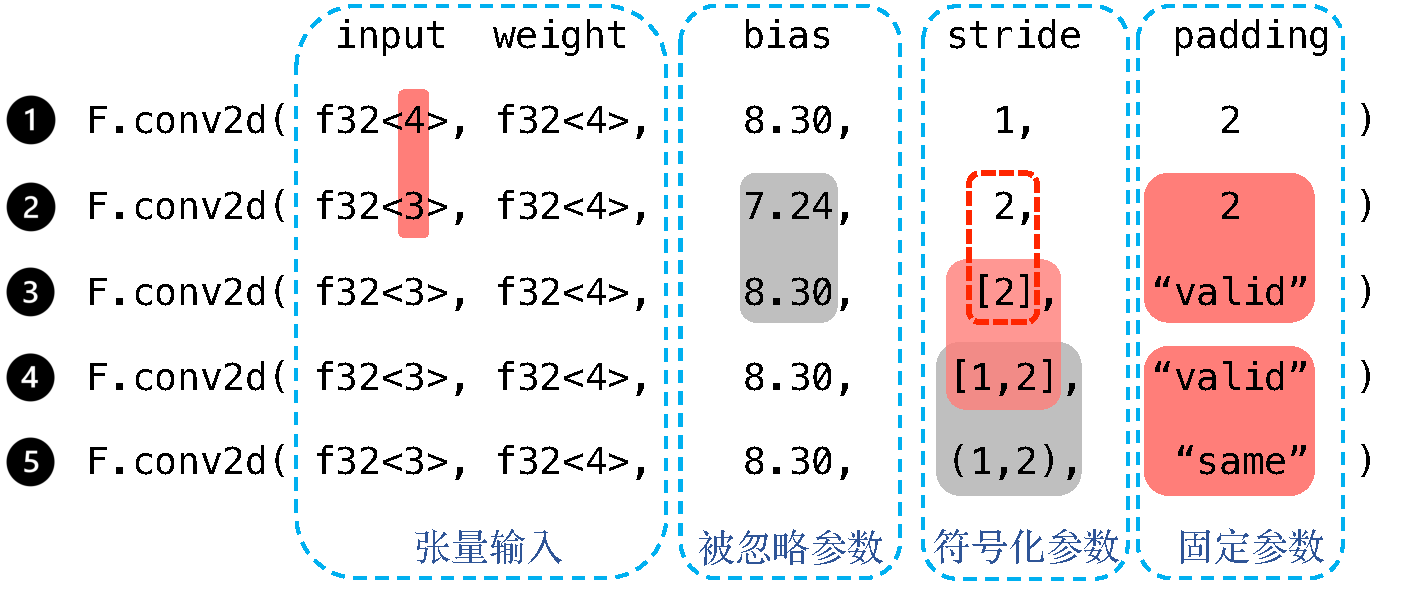
\includegraphics[width=1.\linewidth]{figures/conv2d.pdf}
    \caption{将二维卷积接口的多个具体算子分类为不同偏算子的示例}
    \label{fig:conv2d}
\end{figure}

\begin{itemize}
    \item 对于所有输入参数,其类型固定。如图 \ref{fig:conv2d} 中的第 2、3 个具体算子,它们的参数 \texttt{stride} 和 \texttt{padding} 都有着不同的类型,因此二者属于不同的偏算子。不过,对于张量、标量、字符串、可遍历容器和数据类型以外的类型,我们认为它们不会影响规则推断,如 \texttt{torch.device} ,因此予以忽略。
    \item 对于张量,其维数固定。如第 1、2 个具体算子,其第一个输入张量 \texttt{input} 的形状分别为 $(N, C, H, W)$ 与 $(C, H, W)$ ,前者维数为 4 而后者维数为 3 ,因此二者属于不同的偏算子。这是为了使张量形状符号化之后符号的个数相同。
    \item 对于字符串和布尔型,其值固定。如第 4、5 个具体算子的 \texttt{padding} 值均为字符串类型,但值不相等,因此二者属于不同的偏算子。这是由于字符串和布尔型的变化对接口行为的影响较大,如果将其符号化并加入偏算子规则的表达,往往需要规则的表达和推断算法支持分支语义,而不仅限于代数运算,难度和复杂度将上升。相比之下,对于整型、浮点型和复数则没有额外要求,如第 2、3 个具体算子的 \texttt{bias} 参数虽然不同,但不是将他们归类为两个偏算子的原因。
    \item 对于可遍历容器,首先递归地正规化为列表类型,然后对其元素进行递归处理。如第 3、4 个具体算子的 \texttt{stride} 参数均为列表,但是其长度不相同,因此二者属于不同的偏算子。第 4、5 个具体算子的 \texttt{stride} 参数类型分别为元组和列表,但是正规化为列表后,每个元素均满足上述要求,因此不是将他们归类为两个偏算子的原因。
\end{itemize}
对于满足上述规则的偏算子,其规则与约束推导相比原接口更加容易。外部合作者仅实现了支持简单语法的推导算法,就可以为大部分算子推导符号化规则与约束,并最终提高模糊测试的覆盖率。

\section{混合算子计算图生成算法}

类比混合执行结合具体执行与符号执行的思想,我们改进 NNSmith 中的计算图生成算法,设计可以同时利用 NNSmith 中的符号化算子与本文工作中的具体算子的混合算子计算图生成算法。

混合执行对符号执行的改进之处在于,不会累积符号化规则直到最后再求解,而是面对难以符号化表达的逻辑,及时进行随机具体化。类似地,我们对 NNSmith 中符号化计算图生成算法的改进之处在于,不会累积符号化规则与约束直至图中节点达到预设值才求解,而是在插入每一个算子时进行及时的随机具体化,每一步插入结束时都能得到一个具体化的计算图。

由于我们对 NNSmith 的计算图生成算法做改进,因而在此不再完整地赘述整体的计算图生成算法,而是介绍对其中前向算子插入逻辑的改动。算法 \ref{algo:hygen} 描述了向计算图 $G$ 中插入一个新算子的过程,其顶层逻辑为随机选择以下两种算子插入模式:
\begin{itemize}
    \item \textbf{插入符号化算子。}符号化算子包括两种: NNSmith 中由人工编写规则定义的符号化算子,和基于本文工作中的偏算子进行规则与约束推理得到的符号化算子。首先我们从全部符号化算子中随机选择一个算子,然后枚举计算图中所有与这个算子的输入张量组合在维数和数据类型上一致的张量组合。因为实验中我们不会生成算子个数大于 10 的计算图,因而此处枚举操作的时间开销不至于过大。接着我们考虑每一个符合要求的张量组合,将其代入选定的算子对输入张量形状的符号约束,并用 SMT 求解器进行求解。如果成功得到了一组解,则据此将选定的算子立即具体化,并插入到计算图中。对比 NNSmith ,此处没有将符号规则与约束累积到最后求解,因此每一步插入前后计算图都是具体化的。
    \item \textbf{插入具体算子。} 具体算子的插入本质上是计算图中已有张量组合与具体算子的输入张量组合之间的匹配。例如,计算图中已有两个 \texttt{float32} 类型的张量,形状分别为 \texttt{[8,4,5,5]} 和 \texttt{[4,4,3,3]} ;而具体算子 \texttt{F.conv2d} 的输入恰好也是 \texttt{float32} 类型的形状分别为 \texttt{[8,4,5,5]} 和 \texttt{[4,4,3,3]} 的张量,于是,便可以将两个已有张量分别作为具体算子 \texttt{F.conv2d} 的两个输入,从而插入一个新的具体算子。一般地,我们枚举计算图中所有的张量组合,组合的枚举可以用全局容器进行缓存优化,在每一步插入新算子后进行更新,以避免冗余计算。对于每一种已经存在的张量组合,我们在具体算子数据集中查找是否有输入张量组合恰好与之一致的算子,若有则将其插入到计算图中。为了提高查找效率,我们提前建立了张量形状与数据类型的不同组合到具体算子的映射。
\end{itemize}

\begin{algorithm}
    \caption{混合算子计算图生成算法中的前向算子插入 \texttt{ForwardInsert($\cdot$)}}
    \label{algo:hygen}
\KwIn{计算图 $G$, 符号化算子集合 $\Phi_s$, 具体算子集合 $\mathcal{C}$}
% \KwOut{具体算子集合 $C$}
\SetKw{KwIs}{is}
\SetKw{Continue}{continue}
\SetKwProg{Fn}{Function}{:}{}

\SetKwFunction{FForwardInsert}{ForwardInsert}
\SetKwFunction{FForwardInsertSymbOp}{ForwardInsertSymbOp}
\SetKwFunction{FForwardInsertConcreteOp}{ForwardInsertConcreteOp}

\Fn{\FForwardInsert{$G$}} {
    \uIf{$\texttt{uniform\_sample(0,1)} < 0.5$} {
        % $\phi_s \gets$ 随机选取一个符号化算子\;
        $\phi_s \gets$ $\Phi_s$\texttt{.sample()}\;
        \texttt{ForwardInsertSymbOp}($G$, $\phi_s$)\;
    }
    \Else{
        \texttt{ForwardInsertConcreteOp}($G$)\;
    }
}

\Fn{\FForwardInsertSymbOp{$G$, $\phi_s$}} {
    % $\mathcal{I} \gets$ $G$ 中所有维数与数据类型与 $\phi_s$ 的输入一致的张量组合
    $\mathcal{I} \gets$ $G$.\texttt{tensor\_combinations}($\phi_s$\texttt{.input.ranks}, $\phi_s$\texttt{.input.dtypes})\;
    \For{$i \in \mathcal{I}$} {
        $m \gets \phi$\texttt{.requires}($i$)\;
        $s \gets$ \texttt{solver.solve}($m$)\;
        \If{$s$} {
            $\phi_c \gets \phi$\texttt{.concretize\_by}($s$)\;
            $G$\texttt{.insert\_consumer}($i, \phi_c$)\;
        }
    }
}

\Fn{\FForwardInsertConcreteOp{$G$}} {
    \For{$t \in G$.\texttt{tensor\_combinations}} {
        $\mathcal{C}_\text{cand} \gets \mathcal{C}$\texttt{.lookup}($t$)\;
        $c \gets \mathcal{C}_\text{cand}$\texttt{.sample()}\;
        $G$\texttt{.insert\_consumer}($t, c$)\;
    }
}

\end{algorithm}

\section{差分测试与漏洞寻找}

与 NNSmith 相同,对每个从计算图生成算法构造出的测例,我们分别在不启用编译器的解释执行模式,和启用编译器的图执行模式下运行,运用差分测试比较其结果。若在任一模式下执行失败,则隐式地寻找到漏洞。若在两种模式下均成功执行,但结果的差距不在误差允许范围内,则显式地寻找到漏洞。

\iffalse
\chapter{数学符号和公式}

\section{数学符号}

中文论文的数学符号默认遵循 GB/T 3102.11—1993《物理科学和技术中使用的数学符号》
\footnote{原 GB 3102.11—1993,自 2017 年 3 月 23 日起,该标准转为推荐性标准。}。
该标准参照采纳 ISO 31-11:1992 \footnote{目前已更新为 ISO 80000-2:2019。},
但是与 \TeX{} 默认的美国数学学会(AMS)的符号习惯有所区别。
具体地来说主要有以下差异:
\begin{enumerate}
  \item 大写希腊字母默认为斜体,如
    \begin{equation*}
      \Gamma \Delta \Theta \Lambda \Xi \Pi \Sigma \Upsilon \Phi \Psi \Omega.
    \end{equation*}
    注意有限增量符号 $\increment$ 固定使用正体,模板提供了 \cs{increment} 命令。
  \item 小于等于号和大于等于号使用倾斜的字形 $\le$、$\ge$。
  \item 积分号使用正体,比如 $\int$、$\oint$。
  \item
    偏微分符号 $\partial$ 使用正体。
  \item
    省略号 \cs{dots} 按照中文的习惯固定居中,比如
    \begin{equation*}
      1, 2, \dots, n \quad 1 + 2 + \dots + n.
    \end{equation*}
  \item
    实部 $\Re$ 和虚部 $\Im$ 的字体使用罗马体。
\end{enumerate}

以上数学符号样式的差异可以在模板中统一设置。
另外国标还有一些与 AMS 不同的符号使用习惯,需要用户在写作时进行处理:
\begin{enumerate}
  \item 数学常数和特殊函数名用正体,如
    \begin{equation*}
      \uppi = 3.14\dots; \quad
      \symup{i}^2 = -1; \quad
      \symup{e} = \lim_{n \to \infty} \left( 1 + \frac{1}{n} \right)^n.
    \end{equation*}
  \item 微分号使用正体,比如 $\dif y / \dif x$。
  \item 向量、矩阵和张量用粗斜体(\cs{symbf}),如 $\symbf{x}$、$\symbf{\Sigma}$、$\symbfsf{T}$。
  \item 自然对数用 $\ln x$ 不用 $\log x$。
\end{enumerate}


英文论文的数学符号使用 \TeX{} 默认的样式。
如果有必要,也可以通过设置 \verb|math-style| 选择数学符号样式。

关于量和单位推荐使用
\href{http://mirrors.ctan.org/macros/latex/contrib/siunitx/siunitx.pdf}{\pkg{siunitx}}
宏包,
可以方便地处理希腊字母以及数字与单位之间的空白,
比如:
\SI{6.4e6}{m},
\SI{9}{\micro\meter},
\si{kg.m.s^{-1}},
\SIrange{10}{20}{\degreeCelsius}。



\section{数学公式}

数学公式可以使用 \env{equation} 和 \env{equation*} 环境。
注意数学公式的引用应前后带括号,通常使用 \cs{eqref} 命令,比如式\eqref{eq:example}。
\begin{equation}
  \frac{1}{2 \uppi \symup{i}} \int_\gamma f = \sum_{k=1}^m n(\gamma; a_k) \mathscr{R}(f; a_k).
  \label{eq:example}
\end{equation}

多行公式尽可能在“=”处对齐,推荐使用 \env{align} 环境。
\begin{align}
  a & = b + c + d + e \\
    & = f + g
\end{align}



\section{数学定理}

定理环境的格式可以使用 \pkg{amsthm} 或者 \pkg{ntheorem} 宏包配置。
用户在导言区载入这两者之一后,模板会自动配置 \env{thoerem}、\env{proof} 等环境。

\begin{theorem}[Lindeberg--Lévy 中心极限定理]
  设随机变量 $X_1, X_2, \dots, X_n$ 独立同分布, 且具有期望 $\mu$ 和有限的方差 $\sigma^2 \ne 0$,
  记 $\bar{X}_n = \frac{1}{n} \sum_{i+1}^n X_i$,则
  \begin{equation}
    \lim_{n \to \infty} P \left(\frac{\sqrt{n} \left( \bar{X}_n - \mu \right)}{\sigma} \le z \right) = \Phi(z),
  \end{equation}
  其中 $\Phi(z)$ 是标准正态分布的分布函数。
\end{theorem}
\begin{proof}
  Trivial.
\end{proof}

同时模板还提供了 \env{assumption}、\env{definition}、\env{proposition}、
\env{lemma}、\env{theorem}、\env{axiom}、\env{corollary}、\env{exercise}、
\env{example}、\env{remar}、\env{problem}、\env{conjecture} 这些相关的环境。
\fi

% !TeX root = ../thuthesis-example.tex

\chapter{计算图中间表示与高级语言代码的相互转换}
\label{chp:eng}

\section{实现动机}

NNSmith 中没有显式地对所生成计算图进行表示,而是用 Python 内置列表存储计算图上的各个算子,用字典存储各个张量,在执行计算图时采用循环语句依次执行列表中的算子。然而,这种用一套通用代码运行所有模型的实现方式存在以下两个问题:
\begin{enumerate}
    \item \textbf{干扰深度学习编译器的正常工作。} 对于高级编程语言描述的深度学习模型,深度学习编译器需先对其进行解析,将其行为建模为计算图,然后对计算图做优化。但在解析高级语言方面,深度学习编译器往往不能支持高级语言的全部语法,而只为其中常用的子集提供支持。然而, NNSmith 中的通用模型执行逻辑较为复杂,除了对张量值进行简单的前向传播以外,还实现了提升数值合法性所需的损失值计算与梯度维护等逻辑,其中引入了较多的自定义类与方法,这对深度学习编译器的解析工作不友好。
    如近期新发布的 PyTorch 2.0 \cite{pt2_release} 中的编译接口 \texttt{torch.compile} ,在对 NNSmith 中的模型运行过程进行编译时,就会因不支持的 Python 语法报错而编译失败,因此 NNSmith 无法对这一新推出的编译框架进行测试。
    \item \textbf{给漏洞检查与汇报等人工后处理带来困难。} 上述 NNSmith 的模型执行过程在 Python 代码的实现上有百余层,并且由于对所有模型的执行通用,无法直观地看出计算图的结构与执行过程。因此,对每个 NNSmith 找到的潜在漏洞,我们不能让深度学习框架的开发者运行一整套复杂的 NNSmith 代码来复现,否则会带来较大负担。相反,我们需要对照 NNSmith 输出的包含算子列表与对应输入输出张量的元信息,手工编写可复现漏洞的、最小化的、可独立运行的代码,将其作为漏洞报告的核心部分提交至开发者团队。然而,人工对每个漏洞依次进行编写最小可复现代码、验证其仍能够触发漏洞、以及收集运行日志的一系列操作较为繁琐,会花费较长时间。
\end{enumerate}
因此,我们需要实现从所生成的计算图,到高级语言描述的、最小可复现代码的转换过程,以清晰直观地呈现可触发漏洞的代码逻辑,并减轻漏洞复现与汇报的人工负担。

此外, NNSmith 从零开始构建计算图,没有利用任何真实世界代码;本文在计算图生成时引入了来自真实世界代码的具体算子,在单个算子层面利用了已存在的代码来构造测例。而未来可以探索的方向之一是在多算子层面利用已经存在的代码,来源包括已被修复漏洞的触发代码中的片段、开源项目中的模型片段、以及 ChatGPT\cite{chatgpt}等大语言模型生成的代码片段等,在这些片段的基础上进行编译,以构造测例。而为了利用已存在代码片段并进行变异操作,需要实现从 Python 代码片段到 NNSmith 中计算图表示的转换过程。

综上,我们需要实现计算图表示与 Python 代码的相互转换。由于这一功能主要对测试 PyTorch 2.0 中的编译器有较大帮助、 PyTorch 框架中的配套支持较为完善、并且 PyTorch 开发团队对我们所汇报漏洞的响应较为积极,因此我们暂时只为 PyTorch 框架实现这一功能。

\section{实现方法}

NNSmith 的开发者近期实现了一种供模糊测试所用的计算图中间表示 GraphIR ,以将模型的生成与变异逻辑与下层具体的深度学习框架解耦。而 PyTorch 的 fx 模块\cite{torch_fx}亦为编译过程所需的计算图提供了一种中间表示,并实现了这种中间表示与 Python 可执行代码之间的相互转换。因此,如图 \ref{fig:convert} 所示,我们只需实现 NNSmith GraphIR 与 PyTorch fx 模块之间的相互转换,便可以实现模糊测试框架中计算图的中间表示与 Python 代码的相互转换。

\begin{figure}
    \centering
    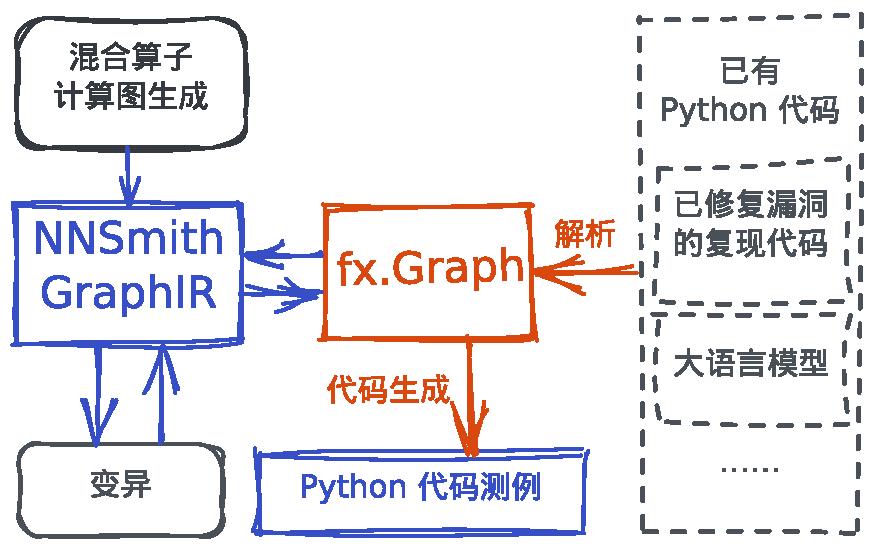
\includegraphics[width=.5\linewidth]{figures/convert.pdf}
    \caption{中间表示与代码间的转换}
    \label{fig:convert}
\end{figure}

\subsection{NNSmith 计算图中间表示简介}

在 NNSmith GraphIR 中,每个计算图由如图 \ref{fig:instir} 所示的若干 InstIR 结构组成。 InstIR 结构包含两部分,分别是输出张量的变量名,和 InstExpr 结构。后者又包括两部分,分别是除了张量输入的其它参数输入都已固定的可调用接口,即算子,与输入张量变量名。之所以将张量输入与其余参数输入分开,是因为在计算图中,我们主要关心的数据流是张量。

\begin{figure}
    \centering
    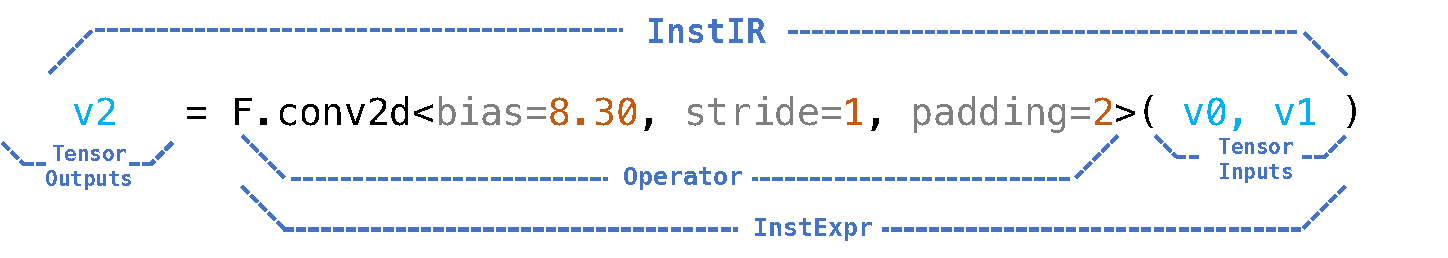
\includegraphics[width=1.\linewidth]{figures/instir.pdf}
    \caption{InstIR 结构示意}
    \label{fig:instir}
\end{figure}

\subsection{PyTorch 计算图中间表示简介}
\label{fxir}

PyTorch 中的 fx 模块提供了计算图的中间表示。如对于代码 \texttt{v = F.conv2d(x, kernel, 8.30, stride=1, padding=2)} , fx 模块可以将其转化为一个中间表示节点,节点上存有以下字段:

\begin{itemize}
    \item \texttt{opcode: call\_function} :意指此节点的操作类型是调用一个函数。
    \item \texttt{name: conv2d} :意为此节点的输出在中间表示中被记为 \texttt{conv2d} 。
    \item \texttt{target: <built-in method conv2d of type object at 0x7f68814c5400>} :存储了此节点所调用的函数的引用。
    \item \texttt{args: (arg0, arg1, tensor)} :列举了调用 \texttt{target} 时的“位置型参数”(positional arguments)。
    \item \texttt{kwargs: {'stride': 1, 'padding': 2}} :列举了调用 \texttt{target} 时的“关键词型参数”(keyword arguments)。
\end{itemize}

可见, PyTorch fx 模块对于接口调用的表示没有以张量数据为中心,只区分了“位置型参数”与“关键词型参数”,而将张量输入与其余输入混合在一起。但是,无论是生成计算图还是对现有计算图做变异,主要考虑的是张量数据的合法匹配问题。因此,相比之下, NNSmith 的计算图中间表示更适用于在模糊测试的背景下操作计算图的场景,为其实现与深度学习框架中的计算图表示之间的转换是值得的。

\subsection{具体实现}

对于给定的进行 PyTorch 张量运算的 Python 代码,我们首先利用 PyTorch 2.0 中推出的 TorchDynamo 模块将其转换为 fx 模块中的计算图。然后,我们遍历已经拓扑排序好的计算图中的各个节点,解析 \ref{fxir} 中介绍的节点上存储的各个字段。我们递归地遍历 \texttt{args} 和 \texttt{kwargs} 两个字段中的每个参数,将张量参数与其余参数分开,从而如图 \ref{fig:instir} 所示,构造其余参数固定的算子,以及输入张量列表,进而形成 \texttt{InstExpr} 结构;然后我们在计算图中新建一个 \texttt{InstIR} 实例,并获取其自动为每个输出张量分配的变量名。由于 fx 模块中的计算图中间表示对变量的命名规则与 NNSmith 不同,因而此处需要根据输出张量在两种中间表示中的不同名称全程维护映射关系,以在后续节点的转化中将 fx 中的输入张量名映射为 NNSmith GraphIR 中的变量名。值得注意的是, fx 模块中间表示中的每个节点均只输出一个变量,对于 \texttt{torch.split} 等输出多变量的节点,会先存为元组,然后通过额外的调用 \texttt{getitem} 方法的节点来获取其中的某个变量。而 NNSmith GraphIR 中表示一个张量操作的 \texttt{InstIR} 结构支持多变量输出,因此我们将做特殊处理,将额外的 \texttt{getitem} 节点压缩至输出多变量的节点中,从而简化计算图的表示,便于对其进行变异。

从 NNSmith GraphIR 向 fx 模块中间表示的转换是上述过程的逆过程,其原理相同且实现类似,因而在此不做赘述。

\section{实现效果}

代码 \ref{listing:nnsmith_forward} 描述了 NNSmith 中前向传播任意模型的实现(删去了为提升数值合法性的逻辑);代码 \ref{listing:gencode} 描述了基于上述 NNSmith GraphIR 到 fx 模块中间表示的转换,再结合 fx 模块从中间表示生成代码的功能,综合出的可独立运行并可复现漏洞的程序。
其中,模型定义中的 \texttt{forward} 函数(第 \ref{listing:gencode:forward} 行)由 fx 模块生成,代码其余部分基于我们定义的模板生成,包括模型定义(第 \ref{listing:gencode:modelinit} 行)、模型权重初始化(第 \ref{listing:gencode:winit} 行)、输入构造(第 \ref{listing:gencode:inputinit} 行)、模型编译(第 \ref{listing:gencode:modelcomp} 行)、解释模式执行(第 \ref{listing:gencode:eagerrun} 行)、编译模式执行(第 \ref{listing:gencode:comprun} 行)与差分测试(第 \ref{listing:gencode:diff} 行)。
可以看出,代码 \ref{listing:gencode} 清晰地描述了具体模型的结构,并能够执行差分测试寻找漏洞,相比前者便于独立运行、修改与调试,可以直接作为漏洞报告的一部分提交至开发者团队。
并且,\ref{sec:bugs_finding} 中为 PyTorch 2.0 寻找到的漏洞绝大部分只能被这种为每个测例单独综合出的程序触发,而不能被 NNSmith 中的通用前向传播函数触发,因此本章工作对漏洞挖掘也具有实际意义。

\begin{listing}[]
    \caption{简化版 NNSmith 前向传播实现}
    \label{listing:nnsmith_forward}
\begin{minted}[
    fontsize=\small,
    linenos, mathescape, escapeinside=||,
    % texcomments,
    frame=lines,
    framesep=1.5mm,    
]{python}
def forward(self, *args, **kwargs):
    tensor_map: Dict[str, torch.Tensor] = {}

    if len(args) == len(self.input_map):
        for i, key in enumerate(self.ir.input_var()):
            tensor_map[key] = args[i]
    elif len(kwargs) == len(self.input_map):
        for ir_key in self.input_map:
            tensor_map[ir_key] = kwargs[ir_key]
    else:
        raise ValueError("Use either args or kwargs only")

    for stmt_idx, instruction in enumerate(self.instructions):
        inst, inps, outs, op = instruction
        input_tensors = [tensor_map[idx] for idx in inps]

        # REAL FORWARD.
        output_tensors = inst(*input_tensors)
        if isinstance(output_tensors, torch.Tensor):
            output_tensors = [output_tensors]
        if isinstance(output_tensors, tuple):
            output_tensors = list(output_tensors)
        output_tensors = output_tensors[: len(op.output_like)]

        for i, out_key in enumerate(outs):
            # put values back to tensor_map.
            tensor_map[out_key] = output_tensors[i]
            
    return tuple(tensor_map[key] for key in self.output_map)
\end{minted}
\end{listing}

\begin{listing}[]
    \caption{从中间表示生成的测例代码}
    \label{listing:gencode}
\begin{minted}[
    fontsize=\small,
    linenos, mathescape, escapeinside=||,
    % texcomments,
    frame=lines,
    framesep=1.5mm,    
]{python}
import numpy as np
import torch
import pickle

# Model definition
class M(torch.nn.Module):
    def __init__(self): |\label{listing:gencode:modelinit}|
        super().__init__()
        self.conv = torch.nn.Conv2d(
            3, 3, kernel_size=(3, 3), stride=(1, 1))
        self.bn = torch.nn.BatchNorm2d(
            3, eps=1e-05, momentum=0.1,
            affine=True, track_running_stats=True)
        self.linear = torch.nn.Linear(
            in_features=62, out_features=3, bias=True)

    def forward(self, x): |\label{listing:gencode:forward}|
        conv = self.conv(x);  x = None
        bn = self.bn(conv);  conv = None
        linear = self.linear(bn);  bn = None
        return linear

m = M()

|\label{listing:gencode:winit}|# Initialize weight
# None

|\label{listing:gencode:inputinit}|# Initialize input
inp = [np.zeros([1, 3, 64, 64], dtype='float32')]

|\label{listing:gencode:modelcomp}|# Compile the model
opt = torch.compile(m, fullgraph=True, backend='inductor')

|\label{listing:gencode:eagerrun}|# Eager run
m_out = m(*[torch.from_numpy(v).to('cpu') for v in inp])
m_out = [v.cpu().detach() for v in m_out] # torch2numpy
m_out = [v.resolve_conj().numpy() if v.is_conj()
    else v.numpy() for v in m_out] # torch2numpy

|\label{listing:gencode:comprun}|# Compiled run
opt_out = opt(*[torch.from_numpy(v).to('cpu') for v in inp])
opt_out = [v.cpu().detach() for v in opt_out] # torch2numpy
opt_out = [v.resolve_conj().numpy() if v.is_conj()
    else v.numpy() for v in opt_out] # torch2numpy

|\label{listing:gencode:diff}|# Differential testing
for i, (l, r) in enumerate(zip(m_out, opt_out)):
    np.testing.assert_allclose(l, r, rtol=1e-2, atol=1e-3,
        err_msg=f"Result mismatch @ index {i}")
\end{minted}
\end{listing}

\iffalse
\chapter{引用文献的标注}

模板支持 BibTeX 和 BibLaTeX 两种方式处理参考文献。
下文主要介绍 BibTeX 配合 \pkg{natbib} 宏包的主要使用方法。


\section{顺序编码制}

在顺序编码制下,默认的 \cs{cite} 命令同 \cs{citep} 一样,序号置于方括号中,
引文页码会放在括号外。
统一处引用的连续序号会自动用短横线连接。

\thusetup{
  cite-style = super,
}
\begin{tabular}{l@{\quad$\Rightarrow$\quad}l}
  \verb|\cite{zhangkun1994}|               & \cite{zhangkun1994}               \\
  \verb|\citet{zhangkun1994}|              & \citet{zhangkun1994}              \\
  \verb|\citep{zhangkun1994}|              & \citep{zhangkun1994}              \\
  \verb|\cite[42]{zhangkun1994}|           & \cite[42]{zhangkun1994}           \\
  \verb|\cite{zhangkun1994,zhukezhen1973}| & \cite{zhangkun1994,zhukezhen1973} \\
\end{tabular}


也可以取消上标格式,将数字序号作为文字的一部分。
建议全文统一使用相同的格式。

\thusetup{
  cite-style = inline,
}
\begin{tabular}{l@{\quad$\Rightarrow$\quad}l}
  \verb|\cite{zhangkun1994}|               & \cite{zhangkun1994}               \\
  \verb|\citet{zhangkun1994}|              & \citet{zhangkun1994}              \\
  \verb|\citep{zhangkun1994}|              & \citep{zhangkun1994}              \\
  \verb|\cite[42]{zhangkun1994}|           & \cite[42]{zhangkun1994}           \\
  \verb|\cite{zhangkun1994,zhukezhen1973}| & \cite{zhangkun1994,zhukezhen1973} \\
\end{tabular}



\section{著者-出版年制}

著者-出版年制下的 \cs{cite} 跟 \cs{citet} 一样。

\thusetup{
  cite-style = author-year,
}
\begin{tabular}{l@{\space$\Rightarrow$\space}l}
  \verb|\cite{zhangkun1994}|                & \cite{zhangkun1994}                \\
  \verb|\citet{zhangkun1994}|               & \citet{zhangkun1994}               \\
  \verb|\citep{zhangkun1994}|               & \citep{zhangkun1994}               \\
  \verb|\cite[42]{zhangkun1994}|            & \cite[42]{zhangkun1994}            \\
  \verb|\citep{zhangkun1994,zhukezhen1973}| & \citep{zhangkun1994,zhukezhen1973} \\
\end{tabular}

\vskip 2ex
\thusetup{
  cite-style = super,
}
注意,引文参考文献的每条都要在正文中标注
\cite{zhangkun1994,zhukezhen1973,dupont1974bone,zhengkaiqing1987,%
  jiangxizhou1980,jianduju1994,merkt1995rotational,mellinger1996laser,%
  bixon1996dynamics,mahui1995,carlson1981two,taylor1983scanning,%
  taylor1981study,shimizu1983laser,atkinson1982experimental,%
  kusch1975perturbations,guangxi1993,huosini1989guwu,wangfuzhi1865songlun,%
  zhaoyaodong1998xinshidai,biaozhunhua2002tushu,chubanzhuanye2004,%
  who1970factors,peebles2001probability,baishunong1998zhiwu,%
  weinstein1974pathogenic,hanjiren1985lun,dizhi1936dizhi,%
  tushuguan1957tushuguanxue,aaas1883science,fugang2000fengsha,%
  xiaoyu2001chubanye,oclc2000about,scitor2000project%
}。
\fi

% !TeX root = ../thuthesis-example.tex

\chapter{实验}
\label{chp:exp}

接下来,本文通过实验对本文提出的方法进行评测,主要关注以下几个问题:

\begin{itemize}
    \item 本文工作可以收集到多少调用记录,从中可以构建多少具体算子?文中提出的偏算子与分类规则,是否能够支持简单的符号规则与约束的自动推导算法?
    \item 对于引入具体算子后的混合算子计算图生成算法,其能否高效地生成合法的计算图,以产生供测试所用的模型?
    \item 基于混合算子计算图生成的模糊测试,其是否在代码分支覆盖数上得到了提升?
    \item 对于本文改进后的模糊测试框架,其是否能够寻找到漏洞?这些漏洞是否可以被前人工作发掘,其质量与实际意义如何?
\end{itemize}

\section{实验设置}

在测试对象上,本文选取了当前最流行的两种深度学习框架 TensorFlow 与 PyTorch 中的编译器。
在与类似工作的比较上,本文主要选择目前效果最好的计算图层面模糊测试框架, NNSmith 。
在实验环境上,本文使用一台 CPU 为 AMD Ryzen Threadripper PRO 5975WX 32-Cores ,内存有 256 GB (3200 MHz),磁盘为 4TB PCIe-4 NVMe SSD ,操作系统为 Ubuntu 22.04.2 LTS 的工作站。
对于算子收集、计算图生成、覆盖率统计实验,本文只考虑在 CPU 上使用 TensorFlow XLA 编译器和 PyTorch JIT 编译器的情况。而在寻找漏洞时,本文包括了在 GPU 上的编译与运行,并引入了两种框架中的其它编译器。

为了统计分支覆盖数,本文需要对深度学习框架进行重新编译。
本文参考 NNSmith 仓库里的覆盖率实验指导\cite{nnsmith_expinstr}进行编译。
对于 PyTorch 框架,本文使用 Clang-14 以及其附带的基于源码的覆盖率统计工具\cite{clang14_cov}编译其 \texttt{2.1.0a0+git6c934a8} 版本。本文较为保守地对可能与 JIT 相关的源码都进行插桩以统计覆盖率。 PyTorch 中与 JIT 相关的代码分散在各处而没有清晰的界限,因此本文粗略地包括了 \texttt{pytorch/csrc} 与 \texttt{aten} 文件夹下的代码。
对于 TensorFlow 框架,本文使用 GCC-9.4 和覆盖率统计工具 GCOV\cite{gcov} 编译其 2.12 开发版 (git hash 前缀为 \texttt{5a6fc0})。本文只对其源码中 \texttt{tensorflow/compiler} 文件夹下的代码进行插桩以统计覆盖率。

\section{具体算子收集}

\begin{table}[]
\centering
\caption{数据收集与整理情况}
\label{tab:opstat}
\begin{tabular}{ccccc}
  \toprule
             & \makecell{收集到轨迹的接口 /\\被插桩接口} & 不重复轨迹 & \makecell{具体算子 /\\具体算子对应的接口} & \makecell{偏算子} \\ \midrule
  PyTorch    & 841 / 1321           & 63144   & 29083 / 678          & 5823  \\
  TensorFlow & 316 / 423            & 34228   & 12908 / 214          & 1799  \\ \bottomrule
\end{tabular}
\end{table}

首先,本文启用 \ref{sec:collect} 中所述的对深度学习框架接口的插桩,按照各自的文档分别运行 PyTorch 的单元测试\cite{pytorch_tests}和 TensorFlow 的单元测试\cite{tf_tests, tf_doctests},从而收集调用轨迹。
表 \ref{tab:opstat} 展示了在插桩、收集、和构建算子过程中的关键数据。

对于 PyTorch ,在全部被插桩的 1323 个接口中,有 841 个(64\%)接口收集到了至少一个调用轨迹; TensorFlow 的这一数值为 316 (75\%)。
二者接口数相差甚远,是因为在 PyTorch 中,有很多“孪生接口”,如 \texttt{Tensor.add} 与它的“就地更改”版本 \texttt{Tensor.add\_} ;还有互为别名的接口,如 \texttt{torch.abs} 与 \texttt{torch.absolute} 。 TensorFlow 中也有类似接口,如 \texttt{tf.raw\_ops.Concat} 与另一个版本 \texttt{tf.raw\_ops.ConcatV2} ,但这种重复与冗余相较 PyTorch 较少。此外, PyTorch 中存在一些复合接口,如 \texttt{Tensor.addbmm} ,而 TensorFlow 中没有这类复合算子。
两个框架均有一部分接口没有收集到任何调用轨迹,很大程度上是因为相互类似的接口的存在。如 \texttt{torch.abs} 被收集到了很多调用轨迹,而 \texttt{torch.absolute} 则没有任何调用轨迹;又如 \texttt{tf.raw\_ops.ConcatV2} 收集到了调用轨迹,而 \texttt{tf.raw\_ops.Concat} 没有。

可以发现,应用 \ref{sec:build_cop} 中的筛选规则后,超过一半的轨迹被丢弃,这主要是因为类似 \texttt{torch.rand\_like} 的接口在单元测试中被大量调用,但不满足确定性要求。根据表中具体算子对应原框架接口的数量可知,分别有 19\% (PyTorch)/ 32\% (TensorFlow)的接口无法通过这一步中的两条检查规则。

最后,应用 \ref{sec:partialop} 中对具体算子的分类规则,可以分别建立 5823 (PyTorch)/ 1799 (TensorFlow)个供符号规则与约束自动推导算法使用的偏算子。基于这些偏算子,外部合作者实现了仅支持加、减、乘、除、最大、最小和模运算的推导算法,就可以为 76\% (PyTorch)/ 84\% (TensorFlow)的偏算子推导出规则与约束。若某接口至少有一个偏算子推导成功就认为这个接口推导成功,则这部分接口占偏算子对应的全部接口的 91\% (PyTorch) / 90\% (TensorFlow) 。若推导成功的接口以符号化算子的形式在混合算子计算图生成中被合法地使用了至少一次就认为对该接口的推导有效,则推导有效的接口占全部参与计算图生成的接口的 96\% (PyTorch) / 96\% (TensorFlow)。可见,本文提出的偏算子概念可以帮助自动推导算法取得较好的效果。

\section{模糊测试用例生成与分支覆盖数}
\label{sec:exp_gen}

对于测例生成,本文比较以下三种不同的计算图生成算法:
\begin{itemize}
    \item NNSmith 中的完全符号化生成算法,记为 NNSmith 。
    \item 同时引入了 NNSmith 中的符号化算子与本文工作中的具体算子的混合算子计算图生成算法,记为 HybridGen-r 。
    \item 利用外部合作者在偏算子上的推导结果,将推导成功的偏算子符号化;在 HybridGen-r 的基础上,保留具体算子的同时,加入这部分通过自动推导建立的符号化算子,进行混合算子计算图生成,记为 HybridGen 。
\end{itemize}
本文限定生成测例的总时间为 4 小时,与前人工作\cite{nnsmith,tzer}保持一致。从后续实验可以看出, 4 小时足够让实验结果基本收敛。

首先,本文考虑如何选取计算图的大小,即图中算子的数量。
图 \ref{fig:covexp:size} 为 HybridGen 算法在 PyTorch 上的消融实验,评价指标(纵轴)为覆盖率,节点数目分别为 1、5、9、13 ,4 小时内每种节点数下生成的合法模型数量标注在图例中。
可以看出,过小的计算图(如单算子计算图)虽然生成速度很快,但会因为无法触发编译器中的图层面优化逻辑(如多算子融合)而只能达到较低的覆盖率,这体现了图层面的模糊测试相比单算子模糊测试的优越性;但计算图大小在增长到一定程度后再继续增大则对提高覆盖率无益,这主要是因为编译器中的优化逻辑一般只涉及到局部几个算子,而不会对较大的子图做优化。
由于目前没有实现在保证漏洞可复现的同时最小化测例的算法,对于较大的计算图构成的测例,发现漏洞后人工进行最小化时的工作量较大。
所以,本文最终选取 5 作为计算图的大小来进行后续实验,以平衡覆盖率效果与人工调试的难度。

其次,本文考察测例生成的效率。
在这一步,本文使用没有为了统计分支覆盖数而在编译时进行插桩的深度学习框架。这是因为在真实场景中进行模糊测试的目的是为了寻找漏洞,而不需要统计分支覆盖数指标,因此只需用官方预编译的普通版本即可。所以在此本文排除插桩带来的额外开销,以反映真实场景中测例生成的效率。
大部分情况下,从一个计算图可以建立一个深度学习模型,从而生成一个测例。但由于在生成计算图时,本文只对张量形状与数据类型做了匹配,而没有考虑输入张量的数值对于算子的合法性,因此会有少量计算图无法被构建为合法的深度学习模型,从而形成一个合法测例。
对此,本文使用解释执行的方式来判断合法性:如果一个计算图对应的模型可以在不启用编译器的解析执行模式下运行成功,则本文认为该计算图合法。
表 \ref{tab:num_tests} 呈现了不同算法在 4 小时内生成的计算图的数量与合法率。
从中可以看出,完全符号化的生成算法 NNSmith 速度最快,且合法率最高。引入了大量具体算子的 HybridGen-r 算法生成速度变慢,且合法率略微下降。这是因为 NNSmith 算法只需考虑 70 余种算子,而 HybridGen-r 算法需要额外考虑上万种具体算子如何被合法地插入计算图,因而时间开销更大;且由于算子种类更多样,合法性更难以保证。至于进一步引入了大量基于自动推导建立的符号算子的 HybridGen 算法,其需要考虑更多算子,且推导出的规则不一定完全正确,因此生成速度与合法性均进一步下降。

\begin{table}[]
\centering
\caption{测例生成情况}
\label{tab:num_tests}
\begin{tabular}{ccccc}
  \toprule
  \multirow{2}{*}{} & \multicolumn{2}{c}{TensorFlow} & \multicolumn{2}{c}{PyTorch} \\ \cmidrule(lr){2-3} \cmidrule(lr){4-5} 
                    & 计算图数量        & 合法率             & 计算图数量      & 合法率            \\ \midrule
  NNSmith           & 139287       & 100.0\%      & 639437     & 100.0\%     \\
  HybridGen-r       & 134120       & 98.1\%      & 410607     & 99.8\%     \\
  HybridGen         & 108572       & 94.8\%      & 208693     & 98.9\%     \\ \bottomrule
\end{tabular}
\end{table}

然后,本文分别在两种框架上对三种计算图生成算法进行源码分支覆盖数评测,以比较不同算法所生成测例的多样性,和基于它们的模糊测试对目标测试的充分程度。
在具体实现上,本文用自编译的为了统计覆盖率而进行了插桩的深度学习框架,对上一步实验中在 4 小时内生成的所有测例用编译执行模式进行重放。
图 \ref{fig:covexp} 表明,在两种框架上, HybridGen-r 均能显著超过 NNSmith ,提升幅度达 13.5\% (PyTorch) / 20.9\% (TensorFlow),证明引入具体算子可以有效提升计算图的多样性。
而对于将具体算子抽象化以提高张量形状多样性的 HybridGen ,则可以进一步提高分支覆盖数,相较 NNSmith 提升幅度达 14.9\% (PyTorch) / 23.5\% (TensorFlow),相较 HybridGen-r 提升幅度达 1.3\% (PyTorch) / 2.2\% (TensorFlow) ,证明了偏算子这一概念可以支撑自动推导算法使深度学习框架与编译器的模糊测试更加充分,为未来工作提供了实现基础与想象空间。

\begin{figure}
    \centering
    \subcaptionbox{PyTorch\label{fig:covexp:pt}}
        {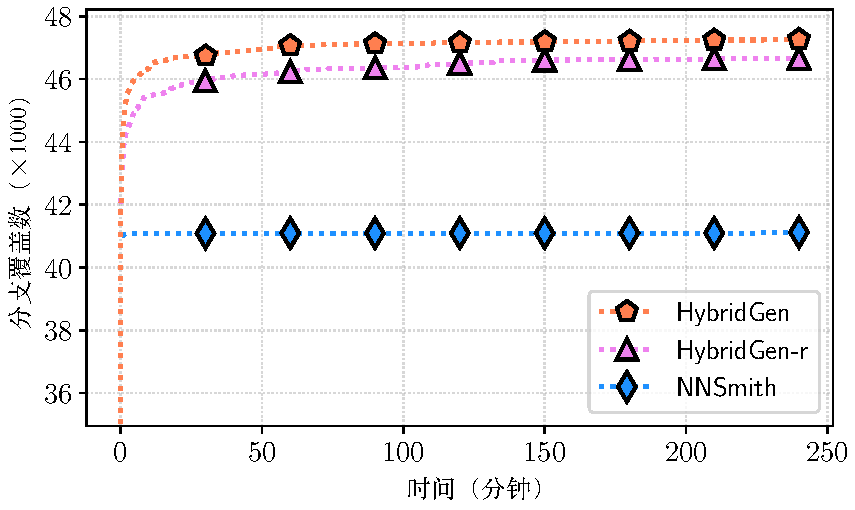
\includegraphics[width=0.48\linewidth]{figures/pt_cov.pdf}}
    \subcaptionbox{TensorFlow\label{fig:covexp:tf}}
        {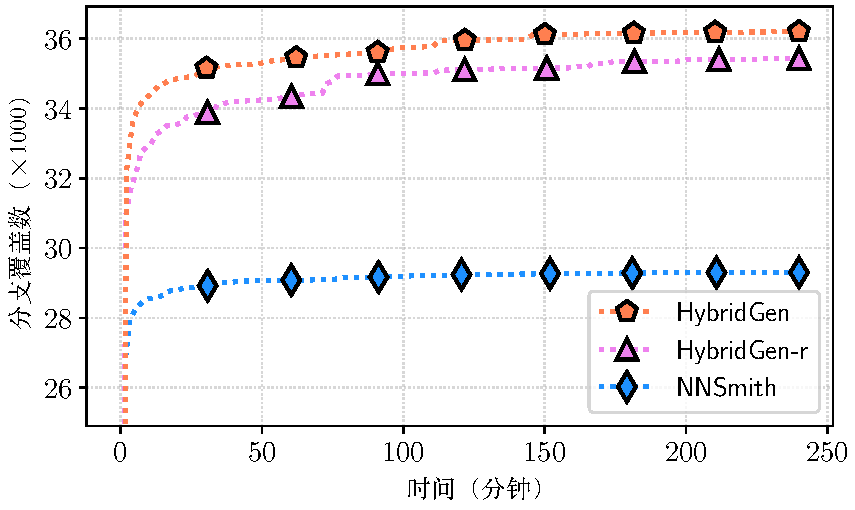
\includegraphics[width=0.48\linewidth]{figures/tf_cov.pdf}}
    \subcaptionbox{模型大小的影响\label{fig:covexp:size}}
        {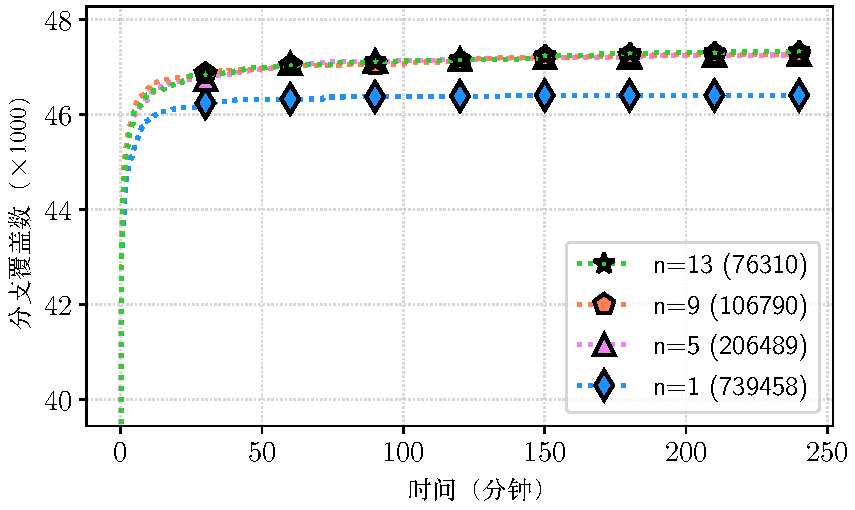
\includegraphics[width=0.48\linewidth]{figures/size_cov.pdf}}
    \caption{模糊测试 4 小时的分支覆盖数变化}
    \label{fig:covexp}
\end{figure}

% PyTorch:
% ----> max cov 41120.0 + max tests 639500
% ----> max cov 46654.0 + max tests 409900  1.1345817121
% ----> max cov 47266.0 + max tests 206500  1.1494649805, 1.0131178463
% TF:
% ----> max cov 29303.0 + max tests 140000
% ----> max cov 35426.0 + max tests 132000  1.2089547145
% ----> max cov 36203.0 + max tests 109000  1.2354707709, 1.0219330435
% Size:
% ----> max cov 46404.0 + max tests 739500
% ----> max cov 47266.0 + max tests 206500
% ----> max cov 47275.0 + max tests 106800
% ----> max cov 47332.0 + max tests 76400

\section{漏洞寻找}
\label{sec:bug_finding}

本文分别在以下设置上运行模糊测试,以寻找潜在漏洞。

\begin{itemize}
    \item TensorFlow: XLA 编译器(包括 CPU 、 GPU)、 TFLite (只支持 CPU);
    \item PyTorch: JIT 编译器、 PyTorch 2.0 编译接口(包括 TorchDynamo 和 TorchInductor)(均包括 CPU 、 GPU)。
\end{itemize}

\subsection{效果概述}

通过不断运行模糊测试框架,并辅以人工筛选与检查,目前本文在开源代码平台 GitHub 上共计向两种框架提交了 76 个被开发团队确认的漏洞。表 \ref{tab:bugs} 从开发团队对漏洞的跟进情况和漏洞的症状两方面进行了统计。
其中, TensorFlow 团队对本文提交的漏洞修复意愿较低,大部分漏洞在确认之后的半年甚至更长时间都没有后续跟进,因而本文逐渐将工作重点放在挖掘 PyTorch 的漏洞上,所以两种框架漏洞总数的差异并不能反映二者可靠性的关系。
对于 PyTorch ,由于开发团队在 2022 年 12 月发布 PyTorch 2.0 后逐渐将工作重点放在了 TorchDynamo 和 TorchInductor 组成的编译技术栈上,而对修复 JIT 编译模块对积极性不强,因此本文在寻找漏洞时也跟随了这一调整。

从表 \ref{tab:bugs} 前 3 列可知,本文提交的绝大部分漏洞都受到了开发者的认可,只有极少数漏洞开发者表示不会进行修复。
对于 PyTorch 团队近期的工作重心 PyTorch 2.0 中的编译技术栈,本文提交的大部分(80.5\%)均已被修复,说明本文提交的漏洞受到重视,具有较高的重要性。
PyTorch 的核心开发者之一在 GitHub 上对本文的工作给予了认可与赞赏,引其原文\cite{ngimel_comments}如下。其表达的主要意思为,本文提交的漏洞并非故意构造而在现实中难以遇到,而是发现了一些可以轻易在实践中被触发,却没有被开发者维护的测试集覆盖的情形。
这段评价不仅体现了本文工作可以生成较为多样的测例,以弥补人工编写的测例集的不足,而且说明了本文构造的测例是在实践中常见的情形,从而具有实际意义。事实上,这两点优势主要均来自于本文在收集具体算子时对真实世界中现有代码的充分利用。

\begin{shadequote}
\small
That said, the bugs you've reported are \textit{high quality}, and as you say, don't look like specially fuzzed set that's impossible to see in practice. They \textit{did} reveal a few common themes that are easy to encounter in practice (even if they are not in our common testing/benchmarking suite), like inplace ops handling (we are working on that), or cpu codegen errors caused by improper use of \texttt{\_\_restrict\_\_} (also working on that).
\end{shadequote}

从表 \ref{tab:bugs} 后 3 列可知,在本文寻找到的漏洞中,报错与错误输出的情况占大多数,而进程崩溃占少数。其中,
“报错”指模型在编译或执行的过程中失败,进程以触发 Python 异常的方式结束;
“错误输出”指模型可以顺利编译与执行,但在没有任何报错的情况下,编译执行模式的输出与解释执行不一致,这在实际应用中可能导致模型在编译之后无法达到先前的效果;
而“进程崩溃”指模型在编译或执行的过程中,进程以非正常的方式结束,如被操作系统强制终止等。
相较“报错”与“进程崩溃”,“错误输出”难以引起用户的注意,因此发现此类漏洞对提升深度学习系统的可靠性具有较强的现实意义。

\begin{table}[]
\centering
\caption{漏洞挖掘情况}
\label{tab:bugs}
\begin{tabular}{ccccccc}
  \toprule
                  & 总计 & 已修复 & 不修复 & 报错                  & 错误输出                & 进程崩溃               \\ \midrule
  PyTorch JIT     & 21 & 8   & 2   & \multirow{2}{*}{39} & \multirow{2}{*}{19} & \multirow{2}{*}{4} \\
  PyTorch 2.0     & 41 & 33  & 0   &                     &                     &                    \\ \cmidrule(lr){1-7} 
  TensorFlow XLA  & 7  & 0   & 1   & \multirow{2}{*}{5}  & \multirow{2}{*}{7}  & \multirow{2}{*}{2} \\
  TensorFlow Lite & 7  & 0   & 0   &                     &                     &                    \\ \bottomrule
\end{tabular}
\end{table}

接下来,本文呈现两个具体漏洞,展示它们的症状表现并分析其根因。

\subsection{底层代码漏洞举例}

PyTorch Issue \#93365\cite{pti93365}是本文提交的被开发团队标记为“high priority”(高优先级)的漏洞之一。
其症状表现为编译后的模型会给出错误的计算结果,具体如代码 \ref{listing:pti93365} 所示。函数 \texttt{fn} 被 PyTorch 2.0 编译后,其返回的第二个张量 \texttt{v1} 被错误地计算为全 0 。(该测例并非模糊测试框架直接给出的原测例,而是经过了后期人工简化,如删去不影响触发漏洞的无关变量和计算等,以便于定位根因。代码 \ref{listing:pti93365} 在原 Issue 的基础上又做了进一步简化,但保持了漏洞的可复现性与根因的一致性。)

\begin{listing}[]
    \caption{PyTorch Issue \#93365 复现代码及报错信息}
    \label{listing:pti93365}
\begin{minted}[
    fontsize=\small,
    linenos, mathescape, escapeinside=||,
    % texcomments,
    frame=lines,
    framesep=1.5mm,    
]{python}
import torch

p0 = torch.tensor([[4.9334, 5.5571]]) # (1, 2)

def fn():
    v7 = torch.cat([p0, p0], dim=0) # v7: (2, 2)
    v1 = torch.mul(v7, v7) # v1: (2, 2)
    return v7, v1

ret_eager = fn()
compiled = torch.compile(fn)
ret_compiled = compiled()

assert torch.allclose(ret_eager[0], ret_compiled[0])
# ^^^ no error
assert torch.allclose(ret_eager[1], ret_compiled[1])
''' ^^^ WRONG!
AssertionError: 
ret_eager[1] =    tensor([[24.3384, 30.8814],
                          [24.3384, 30.8814]])
ret_compiled[1] = tensor([[0., 0.],
                          [0., 0.]])
'''
\end{minted}
\end{listing}

通过追踪与分析开发团队的讨论与修复方式可知,该错误的根因来自底层 C++ 关键字 \texttt{\_\_restrict\_\_} 的错误使用,本文认为其属于底层代码漏洞。
具体来说,对于 Python 语言描述的包含两条 CPU 计算语句的函数 \texttt{fn} , PyTorch 2.0 会将其编译为一个 C++ 语言实现的底层核函数 \texttt{kernel} ,如代码 \ref{listing:pti93365_cpp} 所示。
(本文在代码中添加了注释,以解释 C++ 层面的变量与计算和 Python 层面的变量与计算之间的对应关系。)
% 首先,该段代码通过两个 \texttt{for} 循环计算 Python 中的 \texttt{cat} 操作,将结果输出至 Python 变量 \texttt{v7} 在 C++ 层面对应的两个数组 \texttt{out\_ptr0} 和 \texttt{out\_ptr1} ,这两个数组各自存储了 \texttt{v7} 的一半数据。
% 其次,该段代码用一个 \texttt{for} 循环计算 Python 中的 \texttt{mul} 操作;输入为数组 \texttt{in\_ptr2} ,对应 Python 中 \texttt{v7} 的全部,而输出为数组 \texttt{out\_ptr2} ,对应 Python 中的 \texttt{v1} 。
分析代码可以发现, Python 层面的两个操作存在数据依赖,即 \texttt{mul} 操作的输入 \texttt{v7} 是前一个 \texttt{cat} 操作的输出。而表现在 C++ 层面, \texttt{mul} 操作的输入为 \texttt{in\_ptr2} ,似乎并非 \texttt{cat} 操作的输出 \texttt{out\_ptr0} 与 \texttt{out\_ptr1} 。
然而实际上, \texttt{out\_ptr0} 指向的是 \texttt{v7} 的前一半数据, \texttt{out\_ptr1} 指向的是 \texttt{v7} 的后一半数据,而 \texttt{in\_ptr2} 指向的是 \texttt{v7} 的全部数据,即 \texttt{out\_ptr0} 和 \texttt{out\_ptr1} 均与 \texttt{in\_ptr2} 发生了数据重叠。
而 C++ 函数的参数列表中,被 \texttt{\_\_restrict\_\_} 关键字标记的指针会被编译器认为不存在“别名”,即该指针指向的内存区域不会被其它名称的指针所指并修改,从而可以优化访存逻辑以提高性能。
PyTorch 的开发者在此过于激进地使用了这一优化,导致 \texttt{\_\_restrict\_\_} 关键字的含义与 \texttt{in\_ptr2} 指向的区域被 \texttt{out\_ptr0} 和 \texttt{out\_ptr1} 所指并发生了修改的实际情况不一致,因此产生了错误。

\begin{listing}[]
    \caption{PyTorch Issue \#93365 复现代码}
    \label{listing:pti93365_cpp}
\begin{minted}[
    fontsize=\small,
    linenos, mathescape, escapeinside=||,
    % texcomments,
    frame=lines,
    framesep=1.5mm,    
]{cpp}
extern "C" void kernel(const float* __restrict__ in_ptr0, // p0
                       const float* __restrict__ in_ptr1, // p0
                       const float* __restrict__ in_ptr2, // v7
                       float* __restrict__ out_ptr0, // v7 的前一半
                       float* __restrict__ out_ptr1, // v7 的后一半
                       float* __restrict__ out_ptr2) // v1
{
    { // cat 计算的一部分:将 p0 中的值复制到 v7 的前一半
        #pragma GCC ivdep
        for(long i0=0; i0<2; i0+=1)
        {
            auto tmp0 = in_ptr0[i0];
            out_ptr0[i0] = tmp0;
        }
    }
    { // cat 计算的一部分:将 p0 中的值复制到 v7 的后一半
        #pragma GCC ivdep
        for(long i0=0; i0<2; i0+=1)
        {
            auto tmp0 = in_ptr1[i0];
            out_ptr1[i0] = tmp0;
        }
    }
    { //  mul 计算:将 v7 与 v7 做元素级相乘,输出至 v1
        #pragma GCC ivdep
        for(long i0=0; i0<4; i0+=1)
        {
            auto tmp0 = in_ptr2[i0];|\label{listing:pti93365_cpp:inptr2}|
            auto tmp1 = tmp0 * tmp0;
            out_ptr2[i0] = tmp1;
        }
    }
}
\end{minted}
\end{listing}

下降到汇编层面上分析,若使用 \texttt{\_\_restrict\_\_} 关键字,则在 X86 平台上编译器可以将代码 \ref{listing:pti93365_cpp} 编译为代码 \ref{listing:pti93365_asm} 所示的汇编指令。前 3 条指令将 \texttt{in\_ptr0} 、 \texttt{in\_ptr1} 、 \texttt{in\_ptr2} 指向的数组从内存分别加载至寄存器,第 4 条指令将 \texttt{in\_ptr0} 的数据写入 \texttt{out\_ptr0} ,第 5 条指令将 \texttt{in\_ptr1} 的数据写入 \texttt{out\_ptr1} ,第 6 条指令将 \texttt{in\_ptr2} 的数据与自己相乘,然后在第 7 条指令将结果存入 \texttt{out\_ptr2} 。
其错误在于,第 4 、 5 条指令实际上修改了第 6 条指令的输入,因此 \texttt{in\_ptr2} 数组需要在做乘法之前重新加载。但 \texttt{\_\_restrict\_\_} 关键字使编译器认为 \texttt{in\_ptr2} 指向的内存区域不会被修改,因此没有加载修改后的值,而是直接使用了之前向寄存器中加载的被修改以前的值。
由于在实际中 \texttt{in\_ptr2} 指向的内存经常为初始值 0 ,因此运行该测例时进行乘法之后的输出也常常为 0 ,产生错误输出。

对于该漏洞,开发者的修复方案为,在编译器 TorchInductor 生成底层 C++ 代码的逻辑中,不向函数参数列表中的指针添加 \texttt{\_\_restrict\_\_} 关键字,通过牺牲潜在的性能提升以保证正确性。

此案例说明,本文工作虽然从上层 Python 接口层面进行模糊测试,但可以寻找到根因位于底层 C++ 代码中的漏洞。
而该漏洞需要两个算子产生数据依赖以触发,体现了在多算子计算图层面进行模糊测试的意义。

\begin{listing}[]
    \caption{代码 \ref{listing:pti93365_cpp} 的一种可能的汇编实现}
    \label{listing:pti93365_asm}
\begin{minted}[
    fontsize=\small,
    linenos, mathescape, escapeinside=||,
    % texcomments,
    frame=lines,
    framesep=1.5mm,    
]{nasm}
movq      (%rdi), %rax      ; auto tmpx = in_ptr0[:]
movq      (%rsi), %r10      ; auto tmpy = in_ptr1[:]
movups    (%rdx), %xmm0     ; auto tmp0 = in_ptr2[i0];
movq      %rax, (%rcx)      ; out_ptr0[:] = tmpx;
movq      %r10, (%r8)       ; out_ptr1[:] = tmpy;
mulps     %xmm0, %xmm0      ; auto tmp1 = tmp0 * tmp0;
movups    %xmm0, (%r9)      ; out_ptr2[:] = tmp1;
retq
\end{minted}
\end{listing}

\subsection{高层代码漏洞举例}

PyTorch Issue \#95181\cite{pti95181}同样是本文为 PyTorch 2.0 编译技术栈寻找到的漏洞之一,而其根因位于整个编译流程的 Python 实现中,因此本文认为其属于高层代码漏洞。
原测例经人工简化后如代码 \ref{listing:pti95181} 所示,只需单个算子即可触发。其症状表现为,编译 \texttt{fn} 函数会失败,并产生报错信息如代码最后的注释所示。

\begin{listing}[]
    \caption{PyTorch Issue \#95181 复现代码及报错信息}
    \label{listing:pti95181}
\begin{minted}[
    fontsize=\tiny,
    linenos, mathescape, escapeinside=||,
    % texcomments,
    frame=lines,
    framesep=1.5mm,    
]{python}
import torch

def fn(x: torch.Tensor):
    return x.sub(other=1, alpha=2)

x = torch.rand([1], dtype=torch.float64) |\label{listing:pti95181:x}|

ret_eager = fn(x)
compiled = torch.compile(fn)
ret_compiled = compiled(x)
''' ^^^
Traceback (most recent call last):
  File "python3.10/site-packages/torch/_dynamo/utils.py", line 1196, in run_node
    return getattr(args[0], node.target)(*args[1:], **kwargs)
  File "python3.10/site-packages/torch/utils/_stats.py", line 20, in wrapper
    return fn(*args, **kwargs)
  File "python3.10/site-packages/torch/_subclasses/fake_tensor.py", line 989, in __torch_dispatch__
    return self.dispatch(func, types, args, kwargs)
  File "python3.10/site-packages/torch/_subclasses/fake_tensor.py", line 1172, in dispatch
    r = func(*args, **kwargs)
  File "python3.10/site-packages/torch/_ops.py", line 284, in __call__
    return self._op(*args, **kwargs or {})
  File "python3.10/site-packages/torch/_prims_common/wrappers.py", line 220, in _fn
    result = fn(*args, **kwargs)
  File "python3.10/site-packages/torch/_prims_common/wrappers.py", line 130, in _fn
    result = fn(**bound.arguments)
  File "python3.10/site-packages/torch/_refs/__init__.py", line 1608, in sub
    return prims.sub(a, b)
  File "python3.10/site-packages/torch/_ops.py", line 284, in __call__
    return self._op(*args, **kwargs or {})
  File "python3.10/site-packages/torch/_prims/__init__.py", line 341, in _elementwise_meta
    utils.check_same_dtype(*args)
  File "python3.10/site-packages/torch/_prims_common/__init__.py", line 1079, in check_same_dtype
    raise RuntimeError(msg)
RuntimeError: Tensor with dtype torch.float32 is not the expected dtype of torch.float64!
'''
\end{minted}
\end{listing}

通过分析报错信息中的调用栈可知,其触发过程分为以下几步:

\begin{enumerate}
    \item 在代码 \ref{listing:pti95181} 第 25 行所指的源码附近,测例中的 Python 内置整型参数 \texttt{b} 被提升为了 Python 内置浮点型。\cite{torch_promarg}
    \item 在代码 \ref{listing:pti95181} 第 27 行所指的源码函数中, \texttt{b} 被更新为其与系数 \texttt{alpha} 的乘积,通过 \texttt{prims.mul(b, alpha)} 实现,其返回值类型是数据类型为 \texttt{float32} 的 PyTorch 张量。\cite{torch_primmul}
    \item 代码 \ref{listing:pti95181} 第 27 行所指的源码函数最后执行 \texttt{prims.sub(a, b)} 以计算最终结果。\cite{torch_primsub}此处传入的参数 \texttt{a} 是数据类型为 \texttt{float64} 的 PyTorch 张量(由于本文在代码 \ref{listing:pti95181} 第 \ref{listing:pti95181:x} 行生成的输入为此类型),与上一步更新后的 \texttt{b} 类型不一致。但在 \texttt{prims.sub} 中,对于两个输入参数均为 PyTorch 张量的情况,有强制数据类型一致性检查,因此编译失败而报错。
\end{enumerate}

对于该错误,开发者最终的修复方案为,在上述第 2 步中,若 \texttt{b} 不是 PyTorch 张量类型,则用语句 \texttt{b = b * alpha} 将其与系数 \texttt{alpha} 相乘,以保持其非 PyTorch 张量类型,而把提升类型至 PyTorch 张量的任务交给 \texttt{prims.sub} 接口,以规避报错。\cite{pti95181_fix}

在此案例中,计算操作 \texttt{x.sub(other=1, alpha=2)} 的用法来自于收集到的具体算子。
对于 NNSmith ,其虽然以符号化的形式将 \texttt{sub} 加入到了算子集合中,但只考虑了 \texttt{other} 参数为张量的用法,因而无法生成该测例以触发由类型提升过程导致的错误。
而本文工作中收集到了 \texttt{other} 参数为 Python 内置整型的用法,将其视为算子的非张量属性参数之一而固定不变,只考虑张量 \texttt{x} 的合法性匹配,因而能够生成此测例。
这体现了对于用法灵活的深度学习框架接口,从真实世界代码中收集多样的常见用法并将其引入模糊测试的用例生成,相比纯粹符号化建模算子的方法可以找到更多漏洞,并且具有较强的实际意义。

% !TeX root = ../thuthesis-example.tex

\chapter{结论}
\label{chp:sum}



% 其他部分
\backmatter

% 插图和附表清单
% 本科生的插图索引和表格索引需要移至正文之后、参考文献前
% \listoffiguresandtables  % 插图和附表清单(仅限研究生)
\listoffigures           % 插图清单
\listoftables            % 附表清单

% 符号对照表
% % !TeX root = ../thuthesis-example.tex

\begin{denotation}[3cm]
  \item[PI] 聚酰亚胺
  \item[MPI] 聚酰亚胺模型化合物,N-苯基邻苯酰亚胺
  \item[PBI] 聚苯并咪唑
  \item[MPBI] 聚苯并咪唑模型化合物,N-苯基苯并咪唑
  \item[PY] 聚吡咙
  \item[PMDA-BDA] 均苯四酸二酐与联苯四胺合成的聚吡咙薄膜
  \item[MPY] 聚吡咙模型化合物
  \item[As-PPT] 聚苯基不对称三嗪
  \item[MAsPPT] 聚苯基不对称三嗪单模型化合物,3,5,6-三苯基-1,2,4-三嗪
  \item[DMAsPPT] 聚苯基不对称三嗪双模型化合物(水解实验模型化合物)
  \item[S-PPT] 聚苯基对称三嗪
  \item[MSPPT] 聚苯基对称三嗪模型化合物,2,4,6-三苯基-1,3,5-三嗪
  \item[PPQ] 聚苯基喹噁啉
  \item[MPPQ] 聚苯基喹噁啉模型化合物,3,4-二苯基苯并二嗪
  \item[HMPI] 聚酰亚胺模型化合物的质子化产物
  \item[HMPY] 聚吡咙模型化合物的质子化产物
  \item[HMPBI] 聚苯并咪唑模型化合物的质子化产物
  \item[HMAsPPT] 聚苯基不对称三嗪模型化合物的质子化产物
  \item[HMSPPT] 聚苯基对称三嗪模型化合物的质子化产物
  \item[HMPPQ] 聚苯基喹噁啉模型化合物的质子化产物
  \item[PDT] 热分解温度
  \item[HPLC] 高效液相色谱(High Performance Liquid Chromatography)
  \item[HPCE] 高效毛细管电泳色谱(High Performance Capillary lectrophoresis)
  \item[LC-MS] 液相色谱-质谱联用(Liquid chromatography-Mass Spectrum)
  \item[TIC] 总离子浓度(Total Ion Content)
  \item[\textit{ab initio}] 基于第一原理的量子化学计算方法,常称从头算法
  \item[DFT] 密度泛函理论(Density Functional Theory)
  \item[$E_a$] 化学反应的活化能(Activation Energy)
  \item[ZPE] 零点振动能(Zero Vibration Energy)
  \item[PES] 势能面(Potential Energy Surface)
  \item[TS] 过渡态(Transition State)
  \item[TST] 过渡态理论(Transition State Theory)
  \item[$\increment G^\neq$] 活化自由能(Activation Free Energy)
  \item[$\kappa$] 传输系数(Transmission Coefficient)
  \item[IRC] 内禀反应坐标(Intrinsic Reaction Coordinates)
  \item[$\nu_i$] 虚频(Imaginary Frequency)
  \item[ONIOM] 分层算法(Our own N-layered Integrated molecular Orbital and molecular Mechanics)
  \item[SCF] 自洽场(Self-Consistent Field)
  \item[SCRF] 自洽反应场(Self-Consistent Reaction Field)
\end{denotation}



% 也可以使用 nomencl 宏包,需要在导言区
% \usepackage{nomencl}
% \makenomenclature

% 在这里输出符号说明
% \printnomenclature[3cm]

% 在正文中的任意为都可以标题
% \nomenclature{PI}{聚酰亚胺}
% \nomenclature{MPI}{聚酰亚胺模型化合物,N-苯基邻苯酰亚胺}
% \nomenclature{PBI}{聚苯并咪唑}
% \nomenclature{MPBI}{聚苯并咪唑模型化合物,N-苯基苯并咪唑}
% \nomenclature{PY}{聚吡咙}
% \nomenclature{PMDA-BDA}{均苯四酸二酐与联苯四胺合成的聚吡咙薄膜}
% \nomenclature{MPY}{聚吡咙模型化合物}
% \nomenclature{As-PPT}{聚苯基不对称三嗪}
% \nomenclature{MAsPPT}{聚苯基不对称三嗪单模型化合物,3,5,6-三苯基-1,2,4-三嗪}
% \nomenclature{DMAsPPT}{聚苯基不对称三嗪双模型化合物(水解实验模型化合物)}
% \nomenclature{S-PPT}{聚苯基对称三嗪}
% \nomenclature{MSPPT}{聚苯基对称三嗪模型化合物,2,4,6-三苯基-1,3,5-三嗪}
% \nomenclature{PPQ}{聚苯基喹噁啉}
% \nomenclature{MPPQ}{聚苯基喹噁啉模型化合物,3,4-二苯基苯并二嗪}
% \nomenclature{HMPI}{聚酰亚胺模型化合物的质子化产物}
% \nomenclature{HMPY}{聚吡咙模型化合物的质子化产物}
% \nomenclature{HMPBI}{聚苯并咪唑模型化合物的质子化产物}
% \nomenclature{HMAsPPT}{聚苯基不对称三嗪模型化合物的质子化产物}
% \nomenclature{HMSPPT}{聚苯基对称三嗪模型化合物的质子化产物}
% \nomenclature{HMPPQ}{聚苯基喹噁啉模型化合物的质子化产物}
% \nomenclature{PDT}{热分解温度}
% \nomenclature{HPLC}{高效液相色谱(High Performance Liquid Chromatography)}
% \nomenclature{HPCE}{高效毛细管电泳色谱(High Performance Capillary lectrophoresis)}
% \nomenclature{LC-MS}{液相色谱-质谱联用(Liquid chromatography-Mass Spectrum)}
% \nomenclature{TIC}{总离子浓度(Total Ion Content)}
% \nomenclature{\textit{ab initio}}{基于第一原理的量子化学计算方法,常称从头算法}
% \nomenclature{DFT}{密度泛函理论(Density Functional Theory)}
% \nomenclature{$E_a$}{化学反应的活化能(Activation Energy)}
% \nomenclature{ZPE}{零点振动能(Zero Vibration Energy)}
% \nomenclature{PES}{势能面(Potential Energy Surface)}
% \nomenclature{TS}{过渡态(Transition State)}
% \nomenclature{TST}{过渡态理论(Transition State Theory)}
% \nomenclature{$\increment G^\neq$}{活化自由能(Activation Free Energy)}
% \nomenclature{$\kappa$}{传输系数(Transmission Coefficient)}
% \nomenclature{IRC}{内禀反应坐标(Intrinsic Reaction Coordinates)}
% \nomenclature{$\nu_i$}{虚频(Imaginary Frequency)}
% \nomenclature{ONIOM}{分层算法(Our own N-layered Integrated molecular Orbital and molecular Mechanics)}
% \nomenclature{SCF}{自洽场(Self-Consistent Field)}
% \nomenclature{SCRF}{自洽反应场(Self-Consistent Reaction Field)}


% 参考文献
\bibliography{ref/refs}  % 参考文献使用 BibTeX 编译
% \printbibliography       % 参考文献使用 BibLaTeX 编译

% 致谢
% !TeX root = ../thuthesis-example.tex

\begin{acknowledgements}
  衷心感谢导师×××教授和物理系××副教授对本人的精心指导。他们的言传身教将使我终生受益。

  在美国麻省理工学院化学系进行九个月的合作研究期间,承蒙 Robert Field 教授热心指导与帮助,不胜感激。

  感谢×××××实验室主任×××教授,以及实验室全体老师和同窗们学的热情帮助和支持!

  本课题承蒙国家自然科学基金资助,特此致谢。
\end{acknowledgements}


% 声明
\statement
% 将签字扫描后的声明文件 scan-statement.pdf 替换原始页面
% \statement[file=scan-statement.pdf]
% 本科生编译生成的声明页默认不加页脚,插入扫描版时再补上;
% 研究生编译生成时有页眉页脚,插入扫描版时不再重复。
% 也可以手动控制是否加页眉页脚
% \statement[page-style=empty]
% \statement[file=scan-statement.pdf, page-style=plain]

% 附录
% 本科生需要将附录放到声明之后,个人简历之前
\appendix
% !TeX root = ../thuthesis-example.tex

\begin{survey}
\label{cha:survey}

\title{Background and Related Works of Fuzzing Deep Learning Libraries}
\maketitle

\tableofcontents

Fuzz testing, or fuzzing, was proposed by Prof. Barton Miller in an operating system course project. They generated random inputs, fed them into several Unix utilities, and saw if there was anything unexpected, such as crashes or wrong outputs. Based on it, people have developed various fuzzing techniques sharing the similar underlying idea to test many software programs, including compilers, graphics libraries, and drivers, to strengthen the reliability of software systems.

As deep learning has been becoming more and more popular in recent years, researchers have realized the importance of the reliability of deep learning libraries, such as PyTorch and TensorFlow, as they are deployed in a variety of applications, and some of them, like self-driving vehicles, are safety-critical scenarios. Therefore, several fuzzing-based testing approaches have been proposed to discover bugs and vulnerabilities hidden inside deep learning libraries, which could be categorized as follows.

\section{API-level Fuzzing}

APIs provided by deep learning libraries are the interface that developers interact with to implement deep learning algorithms. Among thousands of these APIs, tensor operation APIs, also tensor operators (e.g. \texttt{torch.add}, \texttt{torch.nn.Linear}), make up the majority, compared with other ones like \texttt{torch.save} and \texttt{torch.optim.Adam}. Tensor operators are the building blocks of deep learning models, thus it is critical to ensure that they are operating as expected. Either crashes or semantic errors could lead to unpleasant consequences when running models, like giving no results or producing wrong results without any warning.

Freefuzz is the first general-purpose and fully automated API-level fuzzing approach for testing popular deep learning libraries, which turns out to be very effective. The whole system can be split into four parts:

\begin{itemize}
    \item \textbf{Code collection.} In order to avoid manual construction of API usage to generate test cases, it collects real-world API usage from unit tests by deep learning developers and open-source projects on GitHub.
    \item \textbf{Instrumentation.} Code in both unit tests and open-source projects cannot be directly used as inputs for testing deep learning libraries, as it only needs a single API invocation each time, and other code needs to be pruned. Thanks to the dynamic typing property of Python, attracting API invocations with all input and output data can be easily achieved by instrumenting a list of deep learning APIs at runtime. In detail, each API can be substituted by a wrapper that will record input/output data in a database so that each invocation can be replayed.
    \item \textbf{Mutation.} Replaying collected API invocations can find some bugs for deep learning compilers, since running successfully in eager mode cannot guarantee success in compiled graph mode. However, to fully utilize existing API usages, mutation is commonly applied in fuzzers to generate highly possible valid test cases with minimum effort. In the scenario of testing deep learning APIs, a variety of attributes may be mutated, such as axis/dimension, tensor shapes, or working modes (e.g. padding modes).
    \item \textbf{Differential Testing.} Exceptions and crashes indicate potential bugs. But for semantic errors like wrong output values, ground truth values are needed to indicate bugs, and values given by eager running mode are always regarded as truth in differential testing as it usually involves nothing related to compilation and optimization.
\end{itemize}

Freefuzz is evaluated in two aspects. 1) Coverage at different levels reflects how much code the testing tool touches. At API-level, Freefuzz tested 470 tensor operation APIs for PyTorch and 688 for TensorFlow. 2) The number of discovered bugs indicates the real-world effectiveness of the testing technique. Freefuzz found 28 bugs for PyTorch and 21 for TensorFlow.

\section{Model-level Fuzzing}

Models are the core of deep learning algorithms, like ResNet for computer vision and Transformers for natural language processing. Models consist of well-connected tensor operators, but improving operators' reliability with API-level fuzzing is not enough to build reliable deep learning systems. It is because of the existence of deep learning compilers, like TVM, XLA, etc., which aim to speed up the inference of large models. A bunch of optimization techniques have been incorporated into these compilers, such as constant folding, operator fusion, and tiling. It is highly possible for developers to make some mistakes when implementing these optimizations, so it is important to test deep learning compilers. But many optimization functions, as listed before, cannot be triggered by a single tensor operator, which reveals the limitation of API-level fuzzing. While single-API invocations can easily be collected with approaches in FreeFuzz, it is non-trivial to get a number of diverse models consisting of multiple tensor operators which will serve as the essential part of oracles for testing deep learning compilers.

For graph-level fuzzers, usually, the more different models they can generate, the higher coverage they can achieve, and the more bugs they can find. There exist several model-level fuzzing works, and among them, NNSmith is the one which can generate the most diverse models. We only focus on three important components of it.

\begin{itemize}
    \item \textbf{Operator Specification} In order to generate models with theoretically arbitrary tensor shapes, NNSmith first defines a symbolic operator set. By "symbolic", it means each operator is modeled by two kinds of symbolic rules, where symbols denote the unknown tensor dimension sizes. 1) Shape transformation rules define how to compute output shapes given input shapes. 2) Shape constraints define the conditions that need to be satisfied by tensor shapes, such as each dimension size should be equal to or greater than zero.
    \item \textbf{Model Generation.} With symbolic defined operators, NNSmith first generates a symbolic graph/model operator by operator, where all tensor shapes are symbolic/uncertain. When inserting a new node/operator, it adds several symbolic constraints to a rule set, including the equivalence between input tensor shapes of this operator and output tensor shapes of its predecessors and the shape constraints in the operator's definition. After inserting a certain amount of nodes/operators, it invokes an SMT solver to assign concrete values to all symbols satisfying all accumulated symbolic rules, turning a symbolic graph into a concrete graph, also a valid input neural network for compilers.
    \item \textbf{Differential Testing.} Like FreeFuzz, NNSmith uses outputs given by the eager running mode as ground truth and compares the outputs produced by the graph/compiled mode with it, to reveal potential bugs of deep learning compilers. Occasionally, the deep learning framework cannot even execute the test case in eager mode, then it indicates a bug unrelated to the compiler but also needs attention.
\end{itemize}

Other similar works (e.g. LEMON, Muffin) cannot generate models as diverse as NNSmith mainly because they are not capable of handling non-shape-preserving operators. It is trivial to build a deep learning model only with shape-preserving operators like element-wise operators (e.g. \texttt{relu}), but that is not the way developers build models for real-world applications. Therefore, a model generator needs to connect different operators with input/output tensors in different shapes while satisfying shape constraints. For example, the output shapes of an operator should be compatible with the input shapes of its successors, which poses challenges. In order to compose valid models with both shape-preserving operators and non-shape-preserving ones, works before NNSmith bypass the shape constraints issue by transforming non-shape-preserving operators to shape-preserving ones with extra layers, including Reshape and Linear, following them. However, this is still not how operators are connected in real-world models, and it also limits the model diversity.

NNSmith, as shown above, can generate very diverse models theoretically. However, in practice, modeling each tensor operator supported by deep learning libraries with handwritten symbolic rules needs tons of human effort. Thus, our work tries to automatically incorporate hundreds of diverse tensor operators to generate deep learning models for testing, which finally turns out to be very effective.


\bibliographystyle{unsrtnat}
\bibliography{ref/appendix}

\end{survey}
       % 本科生:外文资料的调研阅读报告
% % !TeX root = ../thuthesis-example.tex

\begin{translation}
\label{cha:translation}

\title{书面翻译题目}
\maketitle

\tableofcontents


本科生的外文资料书面翻译。


\section{图表示例}

\subsection{图}

附录中的图片示例(图~\ref{fig:appendix-translation-figure})。

\begin{figure}
  \centering
  
\includegraphics[width=0.6\linewidth]{example-image-a.pdf}
  \caption{附录中的图片示例}
  \label{fig:appendix-translation-figure}
\end{figure}


\subsection{表格}

附录中的表格示例(表~\ref{tab:appendix-translation-table})。

\begin{table}
  \centering
  \caption{附录中的表格示例}
  \begin{tabular}{ll}
    \toprule
    文件名          & 描述                         \\
    \midrule
    thuthesis.dtx   & 模板的源文件,包括文档和注释 \\
    thuthesis.cls   & 模板文件                     \\
    thuthesis-*.bst & BibTeX 参考文献表样式文件    \\
    thuthesis-*.bbx & BibLaTeX 参考文献表样式文件  \\
    thuthesis-*.cbx & BibLaTeX 引用样式文件        \\
    \bottomrule
  \end{tabular}
  \label{tab:appendix-translation-table}
\end{table}


\section{数学公式}

附录中的数学公式示例(公式\eqref{eq:appendix-translation-equation})。
\begin{equation}
  \frac{1}{2 \uppi \symup{i}} \int_\gamma f = \sum_{k=1}^m n(\gamma; a_k) \mathscr{R}(f; a_k)
  \label{eq:appendix-translation-equation}
\end{equation}


\section{文献引用}

文献引用示例\cite{abrahams99tex}。


\appendix

\section{附录}

附录的内容。


% 书面翻译的参考文献
\bibliographystyle{unsrtnat}
\bibliography{ref/appendix}

% 书面翻译对应的原文索引
\begin{translation-index}
  \nocite{salomon1995advanced}
  \bibliographystyle{unsrtnat}
  \bibliography{ref/appendix}
\end{translation-index}

\end{translation}
  % 本科生:外文资料的书面翻译
% % !TeX root = ../thuthesis-example.tex

\chapter{补充内容}

附录是与论文内容密切相关、但编入正文又影响整篇论文编排的条理和逻辑性的资料,例如某些重要的数据表格、计算程序、统计表等,是论文主体的补充内容,可根据需要设置。


\section{图表示例}

\subsection{图}

附录中的图片示例(图~\ref{fig:appendix-figure})。

\begin{figure}
  \centering
  
\includegraphics[width=0.6\linewidth]{example-image-a.pdf}
  \caption{附录中的图片示例}
  \label{fig:appendix-figure}
\end{figure}


\subsection{表格}

附录中的表格示例(表~\ref{tab:appendix-table})。

\begin{table}
  \centering
  \caption{附录中的表格示例}
  \begin{tabular}{ll}
    \toprule
    文件名          & 描述                         \\
    \midrule
    thuthesis.dtx   & 模板的源文件,包括文档和注释 \\
    thuthesis.cls   & 模板文件                     \\
    thuthesis-*.bst & BibTeX 参考文献表样式文件    \\
    thuthesis-*.bbx & BibLaTeX 参考文献表样式文件  \\
    thuthesis-*.cbx & BibLaTeX 引用样式文件        \\
    \bottomrule
  \end{tabular}
  \label{tab:appendix-table}
\end{table}


\section{数学公式}

附录中的数学公式示例(公式\eqref{eq:appendix-equation})。
\begin{equation}
  \frac{1}{2 \uppi \symup{i}} \int_\gamma f = \sum_{k=1}^m n(\gamma; a_k) \mathscr{R}(f; a_k)
  \label{eq:appendix-equation}
\end{equation}


% 个人简历、在学期间完成的相关学术成果
% 本科生可以附个人简历,也可以不附个人简历
% % !TeX root = ../thuthesis-example.tex

\begin{resume}

  \section*{个人简历}

  197× 年 ×× 月 ×× 日出生于四川××县。

  1992 年 9 月考入××大学化学系××化学专业,1996 年 7 月本科毕业并获得理学学士学位。

  1996 年 9 月免试进入清华大学化学系攻读××化学博士至今。


  \section*{在学期间完成的相关学术成果}

  \subsection*{学术论文}

  \begin{achievements}
    \item Yang Y, Ren T L, Zhang L T, et al. Miniature microphone with silicon-based ferroelectric thin films[J]. Integrated Ferroelectrics, 2003, 52:229-235.
    \item 杨轶, 张宁欣, 任天令, 等. 硅基铁电微声学器件中薄膜残余应力的研究[J]. 中国机械工程, 2005, 16(14):1289-1291.
    \item 杨轶, 张宁欣, 任天令, 等. 集成铁电器件中的关键工艺研究[J]. 仪器仪表学报, 2003, 24(S4):192-193.
    \item Yang Y, Ren T L, Zhu Y P, et al. PMUTs for handwriting recognition. In press[J]. (已被Integrated Ferroelectrics录用)
  \end{achievements}


  \subsection*{专利}

  \begin{achievements}
    \item 任天令, 杨轶, 朱一平, 等. 硅基铁电微声学传感器畴极化区域控制和电极连接的方法: 中国, CN1602118A[P]. 2005-03-30.
    \item Ren T L, Yang Y, Zhu Y P, et al. Piezoelectric micro acoustic sensor based on ferroelectric materials: USA, No.11/215, 102[P]. (美国发明专利申请号.)
  \end{achievements}

\end{resume}


% 指导教师/指导小组评语
% 本科生不需要
% % !TeX root = ../thuthesis-example.tex

\begin{comments}
% \begin{comments}[name = {指导小组评语}]
% \begin{comments}[name = {Comments from Thesis Supervisor}]
% \begin{comments}[name = {Comments from Thesis Supervision Committee}]

  论文提出了……

\end{comments}


% 答辩委员会决议书
% 本科生不需要
% % !TeX root = ../thuthesis-example.tex

\begin{resolution}

  论文提出了……

  论文取得的主要创新性成果包括:

  1. ……

  2. ……

  3. ……

  论文工作表明作者在×××××具有×××××知识,具有××××能力,论文××××,答辩××××。

  答辩委员会表决,(×票/一致)同意通过论文答辩,并建议授予×××(姓名)×××(门类)学博士/硕士学位。

\end{resolution}


% 本科生的综合论文训练记录表(扫描版)
\record{file=scan-record.pdf}

\end{document}
